\documentclass[twoside]{book}

% Packages required by doxygen
\usepackage{fixltx2e}
\usepackage{calc}
\usepackage{doxygen}
\usepackage[export]{adjustbox} % also loads graphicx
\usepackage{graphicx}
\usepackage[utf8]{inputenc}
\usepackage{makeidx}
\usepackage{multicol}
\usepackage{multirow}
\PassOptionsToPackage{warn}{textcomp}
\usepackage{textcomp}
\usepackage[nointegrals]{wasysym}
\usepackage[table]{xcolor}

% Font selection
\usepackage[T1]{fontenc}
\usepackage[scaled=.90]{helvet}
\usepackage{courier}
\usepackage{amssymb}
\usepackage{sectsty}
\renewcommand{\familydefault}{\sfdefault}
\allsectionsfont{%
  \fontseries{bc}\selectfont%
  \color{darkgray}%
}
\renewcommand{\DoxyLabelFont}{%
  \fontseries{bc}\selectfont%
  \color{darkgray}%
}
\newcommand{\+}{\discretionary{\mbox{\scriptsize$\hookleftarrow$}}{}{}}

% Page & text layout
\usepackage{geometry}
\geometry{%
  a4paper,%
  top=2.5cm,%
  bottom=2.5cm,%
  left=2.5cm,%
  right=2.5cm%
}
\tolerance=750
\hfuzz=15pt
\hbadness=750
\setlength{\emergencystretch}{15pt}
\setlength{\parindent}{0cm}
\setlength{\parskip}{3ex plus 2ex minus 2ex}
\makeatletter
\renewcommand{\paragraph}{%
  \@startsection{paragraph}{4}{0ex}{-1.0ex}{1.0ex}{%
    \normalfont\normalsize\bfseries\SS@parafont%
  }%
}
\renewcommand{\subparagraph}{%
  \@startsection{subparagraph}{5}{0ex}{-1.0ex}{1.0ex}{%
    \normalfont\normalsize\bfseries\SS@subparafont%
  }%
}
\makeatother

% Headers & footers
\usepackage{fancyhdr}
\pagestyle{fancyplain}
\fancyhead[LE]{\fancyplain{}{\bfseries\thepage}}
\fancyhead[CE]{\fancyplain{}{}}
\fancyhead[RE]{\fancyplain{}{\bfseries\leftmark}}
\fancyhead[LO]{\fancyplain{}{\bfseries\rightmark}}
\fancyhead[CO]{\fancyplain{}{}}
\fancyhead[RO]{\fancyplain{}{\bfseries\thepage}}
\fancyfoot[LE]{\fancyplain{}{}}
\fancyfoot[CE]{\fancyplain{}{}}
\fancyfoot[RE]{\fancyplain{}{\bfseries\scriptsize Generated by Doxygen }}
\fancyfoot[LO]{\fancyplain{}{\bfseries\scriptsize Generated by Doxygen }}
\fancyfoot[CO]{\fancyplain{}{}}
\fancyfoot[RO]{\fancyplain{}{}}
\renewcommand{\footrulewidth}{0.4pt}
\renewcommand{\chaptermark}[1]{%
  \markboth{#1}{}%
}
\renewcommand{\sectionmark}[1]{%
  \markright{\thesection\ #1}%
}

% Indices & bibliography
\usepackage{natbib}
\usepackage[titles]{tocloft}
\setcounter{tocdepth}{3}
\setcounter{secnumdepth}{5}
\makeindex

% Hyperlinks (required, but should be loaded last)
\usepackage{ifpdf}
\ifpdf
  \usepackage[pdftex,pagebackref=true]{hyperref}
\else
  \usepackage[ps2pdf,pagebackref=true]{hyperref}
\fi
\hypersetup{%
  colorlinks=true,%
  linkcolor=blue,%
  citecolor=blue,%
  unicode%
}

% Custom commands
\newcommand{\clearemptydoublepage}{%
  \newpage{\pagestyle{empty}\cleardoublepage}%
}

\usepackage{caption}
\captionsetup{labelsep=space,justification=centering,font={bf},singlelinecheck=off,skip=4pt,position=top}

%===== C O N T E N T S =====

\begin{document}

% Titlepage & ToC
\hypersetup{pageanchor=false,
             bookmarksnumbered=true,
             pdfencoding=unicode
            }
\pagenumbering{roman}
\begin{titlepage}
\vspace*{7cm}
\begin{center}%
{\Large Naval Battles \\[1ex]\large 0.\+3.\+9 }\\
\vspace*{1cm}
{\large Generated by Doxygen 1.8.11}\\
\end{center}
\end{titlepage}
\clearemptydoublepage
\tableofcontents
\clearemptydoublepage
\pagenumbering{arabic}
\hypersetup{pageanchor=true}

%--- Begin generated contents ---
\chapter{Naval Battles}
\label{md_C:_Users_Piotr_Desktop_CLion_proj_naval_battles_README}
\hypertarget{md_C:_Users_Piotr_Desktop_CLion_proj_naval_battles_README}{}
\input{md_C:_Users_Piotr_Desktop_CLion_proj_naval_battles_README}
\chapter{Hierarchical Index}
\section{Class Hierarchy}
This inheritance list is sorted roughly, but not completely, alphabetically\+:\begin{DoxyCompactList}
\item \contentsline{section}{Battle}{\pageref{class_battle}}{}
\item \contentsline{section}{Parameters}{\pageref{struct_parameters}}{}
\item \contentsline{section}{Ship}{\pageref{class_ship}}{}
\begin{DoxyCompactList}
\item \contentsline{section}{Aircraft\+Carrier}{\pageref{class_aircraft_carrier}}{}
\item \contentsline{section}{Battleship}{\pageref{class_battleship}}{}
\item \contentsline{section}{Cruiser}{\pageref{class_cruiser}}{}
\item \contentsline{section}{Destroyer}{\pageref{class_destroyer}}{}
\end{DoxyCompactList}
\item \contentsline{section}{site}{\pageref{structsite}}{}
\end{DoxyCompactList}

\chapter{Class Index}
\section{Class List}
Here are the classes, structs, unions and interfaces with brief descriptions\+:\begin{DoxyCompactList}
\item\contentsline{section}{\hyperlink{class_aircraft_carrier}{Aircraft\+Carrier} }{\pageref{class_aircraft_carrier}}{}
\item\contentsline{section}{\hyperlink{class_battle}{Battle} }{\pageref{class_battle}}{}
\item\contentsline{section}{\hyperlink{class_battleship}{Battleship} }{\pageref{class_battleship}}{}
\item\contentsline{section}{\hyperlink{class_cruiser}{Cruiser} }{\pageref{class_cruiser}}{}
\item\contentsline{section}{\hyperlink{class_destroyer}{Destroyer} }{\pageref{class_destroyer}}{}
\item\contentsline{section}{\hyperlink{struct_parameters}{Parameters} }{\pageref{struct_parameters}}{}
\item\contentsline{section}{\hyperlink{class_ship}{Ship} }{\pageref{class_ship}}{}
\item\contentsline{section}{\hyperlink{structsite}{site} }{\pageref{structsite}}{}
\end{DoxyCompactList}

\chapter{File Index}
\section{File List}
Here is a list of all files with brief descriptions\+:\begin{DoxyCompactList}
\item\contentsline{section}{C\+:/\+Users/\+Piotr/\+Desktop/\+C\+Lion/proj\+\_\+naval\+\_\+battles/\hyperlink{_battle_8cpp}{Battle.\+cpp} }{\pageref{_battle_8cpp}}{}
\item\contentsline{section}{C\+:/\+Users/\+Piotr/\+Desktop/\+C\+Lion/proj\+\_\+naval\+\_\+battles/\hyperlink{_battle_8h}{Battle.\+h} }{\pageref{_battle_8h}}{}
\item\contentsline{section}{C\+:/\+Users/\+Piotr/\+Desktop/\+C\+Lion/proj\+\_\+naval\+\_\+battles/\hyperlink{_functions_8cpp}{Functions.\+cpp} }{\pageref{_functions_8cpp}}{}
\item\contentsline{section}{C\+:/\+Users/\+Piotr/\+Desktop/\+C\+Lion/proj\+\_\+naval\+\_\+battles/\hyperlink{_functions_8h}{Functions.\+h} }{\pageref{_functions_8h}}{}
\item\contentsline{section}{C\+:/\+Users/\+Piotr/\+Desktop/\+C\+Lion/proj\+\_\+naval\+\_\+battles/\hyperlink{main_8cpp}{main.\+cpp} }{\pageref{main_8cpp}}{}
\item\contentsline{section}{C\+:/\+Users/\+Piotr/\+Desktop/\+C\+Lion/proj\+\_\+naval\+\_\+battles/\hyperlink{_ship_8cpp}{Ship.\+cpp} }{\pageref{_ship_8cpp}}{}
\item\contentsline{section}{C\+:/\+Users/\+Piotr/\+Desktop/\+C\+Lion/proj\+\_\+naval\+\_\+battles/\hyperlink{_ship_8h}{Ship.\+h} }{\pageref{_ship_8h}}{}
\end{DoxyCompactList}

\chapter{Class Documentation}
\hypertarget{class_aircraft_carrier}{}\section{Aircraft\+Carrier Class Reference}
\label{class_aircraft_carrier}\index{Aircraft\+Carrier@{Aircraft\+Carrier}}


{\ttfamily \#include $<$Ship.\+h$>$}

Inheritance diagram for Aircraft\+Carrier\+:\begin{figure}[H]
\begin{center}
\leavevmode
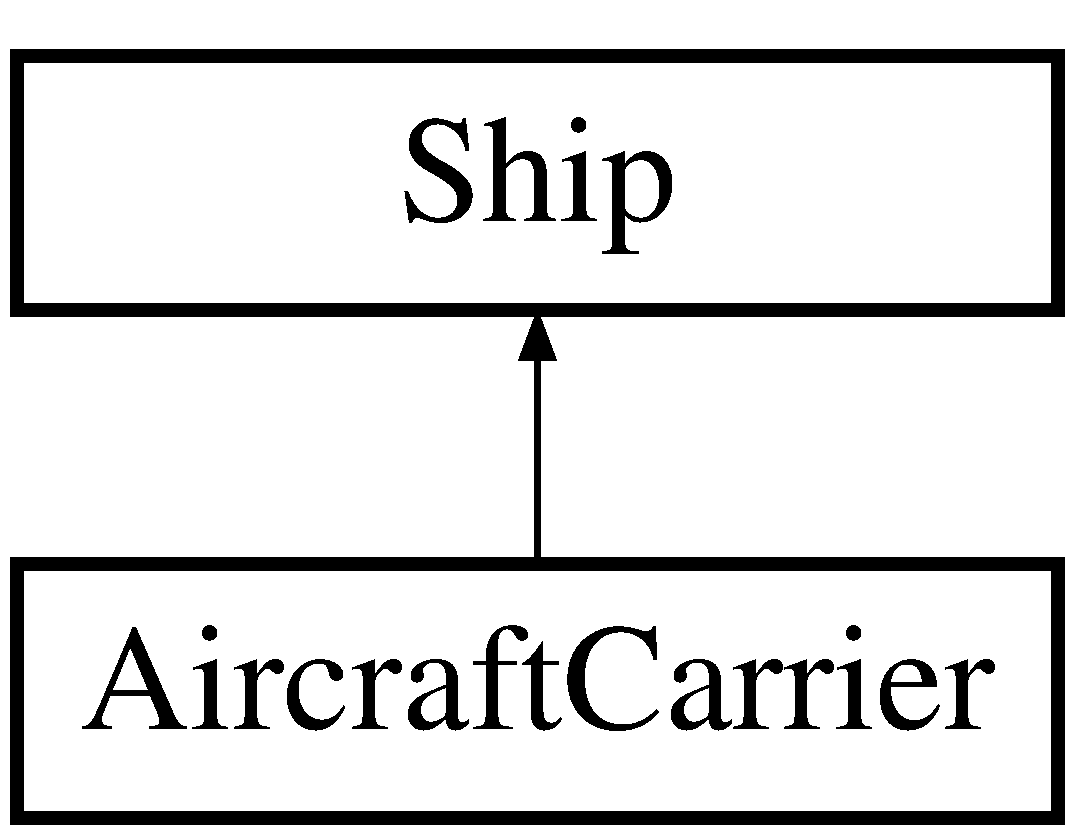
\includegraphics[height=2.000000cm]{class_aircraft_carrier}
\end{center}
\end{figure}
\subsection*{Public Member Functions}
\begin{DoxyCompactItemize}
\item 
\hyperlink{class_aircraft_carrier_a34bd9eb88f293611e422b824e031f70f}{Aircraft\+Carrier} (\hyperlink{struct_parameters}{Parameters} parameters\mbox{[}$\,$\mbox{]}, unsigned int i)
\item 
virtual void \hyperlink{class_aircraft_carrier_a6a4f9376d570301e2a720d699d61af1c}{attack} ()
\item 
unsigned int \hyperlink{class_aircraft_carrier_a1521dc1e79308c4ebd1b979a48878446}{number\+Of\+Squadrons} ()
\end{DoxyCompactItemize}
\subsection*{Additional Inherited Members}


\subsection{Constructor \& Destructor Documentation}
\index{Aircraft\+Carrier@{Aircraft\+Carrier}!Aircraft\+Carrier@{Aircraft\+Carrier}}
\index{Aircraft\+Carrier@{Aircraft\+Carrier}!Aircraft\+Carrier@{Aircraft\+Carrier}}
\subsubsection[{\texorpdfstring{Aircraft\+Carrier(\+Parameters parameters[], unsigned int i)}{AircraftCarrier(Parameters parameters[], unsigned int i)}}]{\setlength{\rightskip}{0pt plus 5cm}Aircraft\+Carrier\+::\+Aircraft\+Carrier (
\begin{DoxyParamCaption}
\item[{{\bf Parameters}}]{parameters\mbox{[}$\,$\mbox{]}, }
\item[{unsigned int}]{i}
\end{DoxyParamCaption}
)}\hypertarget{class_aircraft_carrier_a34bd9eb88f293611e422b824e031f70f}{}\label{class_aircraft_carrier_a34bd9eb88f293611e422b824e031f70f}


\subsection{Member Function Documentation}
\index{Aircraft\+Carrier@{Aircraft\+Carrier}!attack@{attack}}
\index{attack@{attack}!Aircraft\+Carrier@{Aircraft\+Carrier}}
\subsubsection[{\texorpdfstring{attack()}{attack()}}]{\setlength{\rightskip}{0pt plus 5cm}virtual void Aircraft\+Carrier\+::attack (
\begin{DoxyParamCaption}
{}
\end{DoxyParamCaption}
)\hspace{0.3cm}{\ttfamily [inline]}, {\ttfamily [virtual]}}\hypertarget{class_aircraft_carrier_a6a4f9376d570301e2a720d699d61af1c}{}\label{class_aircraft_carrier_a6a4f9376d570301e2a720d699d61af1c}


Implements \hyperlink{class_ship_a75d4d83e8f6bbaf06be9d1bf45c2bdd5}{Ship}.

\index{Aircraft\+Carrier@{Aircraft\+Carrier}!number\+Of\+Squadrons@{number\+Of\+Squadrons}}
\index{number\+Of\+Squadrons@{number\+Of\+Squadrons}!Aircraft\+Carrier@{Aircraft\+Carrier}}
\subsubsection[{\texorpdfstring{number\+Of\+Squadrons()}{numberOfSquadrons()}}]{\setlength{\rightskip}{0pt plus 5cm}unsigned int Aircraft\+Carrier\+::number\+Of\+Squadrons (
\begin{DoxyParamCaption}
{}
\end{DoxyParamCaption}
)\hspace{0.3cm}{\ttfamily [inline]}, {\ttfamily [virtual]}}\hypertarget{class_aircraft_carrier_a1521dc1e79308c4ebd1b979a48878446}{}\label{class_aircraft_carrier_a1521dc1e79308c4ebd1b979a48878446}


Implements \hyperlink{class_ship_abc3639e150f87a41a4ac1b770db7b56a}{Ship}.



The documentation for this class was generated from the following files\+:\begin{DoxyCompactItemize}
\item 
C\+:/\+Users/\+Piotr/\+Desktop/\+C\+Lion/proj\+\_\+naval\+\_\+battles/\hyperlink{_ship_8h}{Ship.\+h}\item 
C\+:/\+Users/\+Piotr/\+Desktop/\+C\+Lion/proj\+\_\+naval\+\_\+battles/\hyperlink{_ship_8cpp}{Ship.\+cpp}\end{DoxyCompactItemize}

\hypertarget{class_battle}{}\section{Battle Class Reference}
\label{class_battle}\index{Battle@{Battle}}


{\ttfamily \#include $<$Battle.\+h$>$}

\subsection*{Public Member Functions}
\begin{DoxyCompactItemize}
\item 
\hyperlink{class_battle_abecc253b23b71da260445e4bdc8522e2}{Battle} ()
\item 
bool \hyperlink{class_battle_a5a078e86f44331d91aa2046020357f03}{main\+Loop} ()
\begin{DoxyCompactList}\small\item\em Create a \hyperlink{class_battle}{Battle}. \end{DoxyCompactList}\item 
int \hyperlink{class_battle_a4f2668e41e3b6aa06d13a82be088350f}{draw\+Ship} (unsigned int n)
\item 
void \hyperlink{class_battle_acc3373dae102937dae66a45f87ee6027}{show\+Sites} ()
\item 
int \hyperlink{class_battle_afefb3ebee903514b1410cc3c65bb62ed}{turn} (int wf)
\end{DoxyCompactItemize}


\subsection{Constructor \& Destructor Documentation}
\index{Battle@{Battle}!Battle@{Battle}}
\index{Battle@{Battle}!Battle@{Battle}}
\subsubsection[{\texorpdfstring{Battle()}{Battle()}}]{\setlength{\rightskip}{0pt plus 5cm}Battle\+::\+Battle (
\begin{DoxyParamCaption}
{}
\end{DoxyParamCaption}
)}\hypertarget{class_battle_abecc253b23b71da260445e4bdc8522e2}{}\label{class_battle_abecc253b23b71da260445e4bdc8522e2}


\subsection{Member Function Documentation}
\index{Battle@{Battle}!draw\+Ship@{draw\+Ship}}
\index{draw\+Ship@{draw\+Ship}!Battle@{Battle}}
\subsubsection[{\texorpdfstring{draw\+Ship(unsigned int n)}{drawShip(unsigned int n)}}]{\setlength{\rightskip}{0pt plus 5cm}int Battle\+::draw\+Ship (
\begin{DoxyParamCaption}
\item[{unsigned int}]{n}
\end{DoxyParamCaption}
)}\hypertarget{class_battle_a4f2668e41e3b6aa06d13a82be088350f}{}\label{class_battle_a4f2668e41e3b6aa06d13a82be088350f}
\index{Battle@{Battle}!main\+Loop@{main\+Loop}}
\index{main\+Loop@{main\+Loop}!Battle@{Battle}}
\subsubsection[{\texorpdfstring{main\+Loop()}{mainLoop()}}]{\setlength{\rightskip}{0pt plus 5cm}bool Battle\+::main\+Loop (
\begin{DoxyParamCaption}
{}
\end{DoxyParamCaption}
)}\hypertarget{class_battle_a5a078e86f44331d91aa2046020357f03}{}\label{class_battle_a5a078e86f44331d91aa2046020357f03}


Create a \hyperlink{class_battle}{Battle}. 

\index{Battle@{Battle}!show\+Sites@{show\+Sites}}
\index{show\+Sites@{show\+Sites}!Battle@{Battle}}
\subsubsection[{\texorpdfstring{show\+Sites()}{showSites()}}]{\setlength{\rightskip}{0pt plus 5cm}void Battle\+::show\+Sites (
\begin{DoxyParamCaption}
{}
\end{DoxyParamCaption}
)}\hypertarget{class_battle_acc3373dae102937dae66a45f87ee6027}{}\label{class_battle_acc3373dae102937dae66a45f87ee6027}
\index{Battle@{Battle}!turn@{turn}}
\index{turn@{turn}!Battle@{Battle}}
\subsubsection[{\texorpdfstring{turn(int wf)}{turn(int wf)}}]{\setlength{\rightskip}{0pt plus 5cm}int Battle\+::turn (
\begin{DoxyParamCaption}
\item[{int}]{wf}
\end{DoxyParamCaption}
)}\hypertarget{class_battle_afefb3ebee903514b1410cc3c65bb62ed}{}\label{class_battle_afefb3ebee903514b1410cc3c65bb62ed}


The documentation for this class was generated from the following files\+:\begin{DoxyCompactItemize}
\item 
C\+:/\+Users/\+Piotr/\+Desktop/\+C\+Lion/proj\+\_\+naval\+\_\+battles/\hyperlink{_battle_8h}{Battle.\+h}\item 
C\+:/\+Users/\+Piotr/\+Desktop/\+C\+Lion/proj\+\_\+naval\+\_\+battles/\hyperlink{_battle_8cpp}{Battle.\+cpp}\end{DoxyCompactItemize}

\hypertarget{class_battleship}{}\section{Battleship Class Reference}
\label{class_battleship}\index{Battleship@{Battleship}}


{\ttfamily \#include $<$Ship.\+h$>$}

Inheritance diagram for Battleship\+:\begin{figure}[H]
\begin{center}
\leavevmode
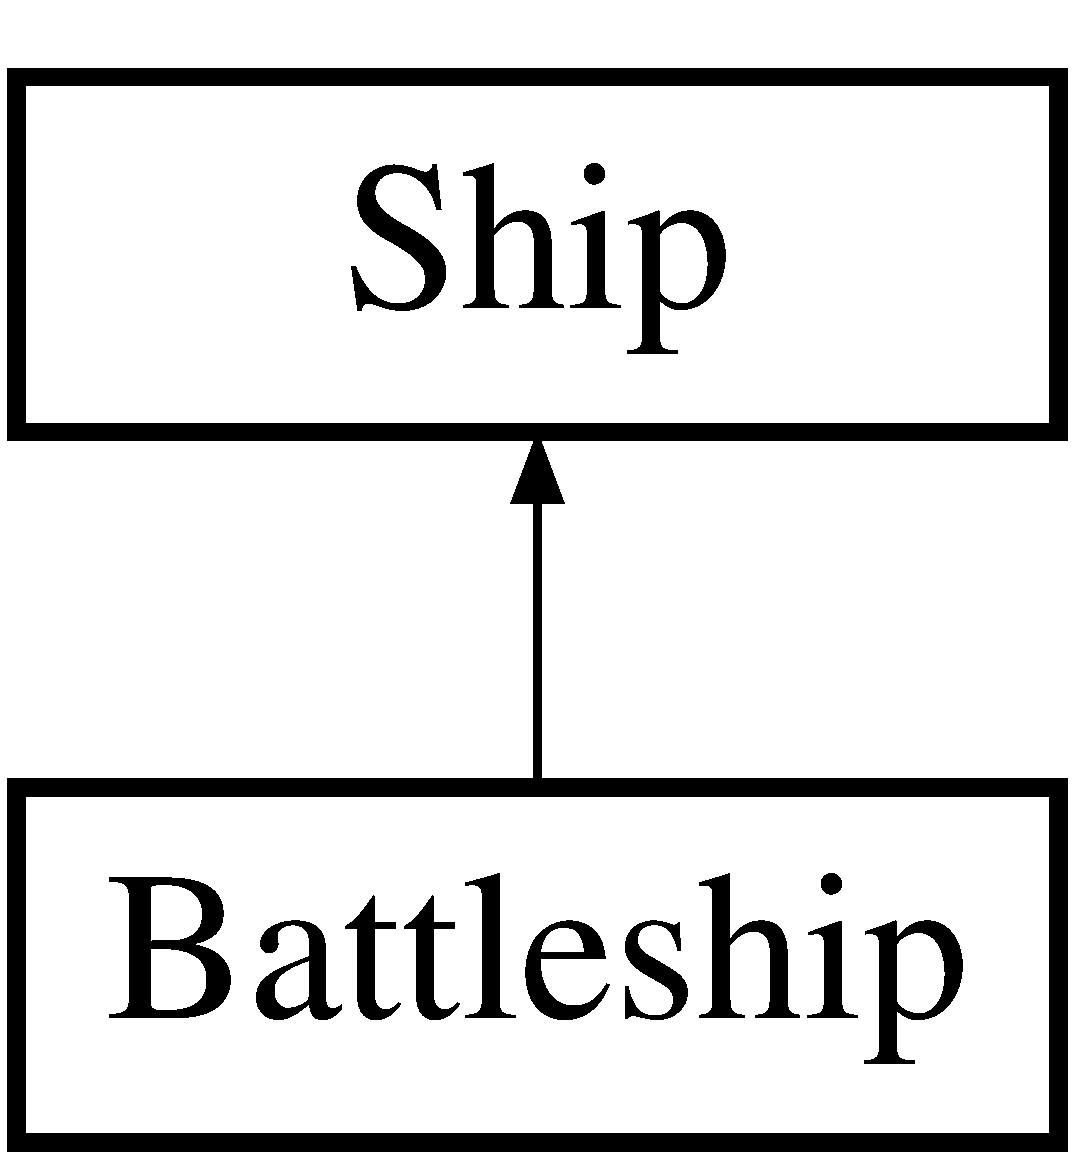
\includegraphics[height=2.000000cm]{class_battleship}
\end{center}
\end{figure}
\subsection*{Public Member Functions}
\begin{DoxyCompactItemize}
\item 
\hyperlink{class_battleship_ae1e567f105c49e38f45e354a4e699d0c}{Battleship} (\hyperlink{struct_parameters}{Parameters} parameters\mbox{[}$\,$\mbox{]}, unsigned int i)
\item 
unsigned int \hyperlink{class_battleship_af64957b1b5dbc5c0fab74c90b94de9d0}{number\+Of\+Squadrons} ()
\item 
virtual void \hyperlink{class_battleship_a599cd8efe7d763b170b1352813cf47f1}{attack} ()
\end{DoxyCompactItemize}
\subsection*{Additional Inherited Members}


\subsection{Constructor \& Destructor Documentation}
\index{Battleship@{Battleship}!Battleship@{Battleship}}
\index{Battleship@{Battleship}!Battleship@{Battleship}}
\subsubsection[{\texorpdfstring{Battleship(\+Parameters parameters[], unsigned int i)}{Battleship(Parameters parameters[], unsigned int i)}}]{\setlength{\rightskip}{0pt plus 5cm}Battleship\+::\+Battleship (
\begin{DoxyParamCaption}
\item[{{\bf Parameters}}]{parameters\mbox{[}$\,$\mbox{]}, }
\item[{unsigned int}]{i}
\end{DoxyParamCaption}
)}\hypertarget{class_battleship_ae1e567f105c49e38f45e354a4e699d0c}{}\label{class_battleship_ae1e567f105c49e38f45e354a4e699d0c}


\subsection{Member Function Documentation}
\index{Battleship@{Battleship}!attack@{attack}}
\index{attack@{attack}!Battleship@{Battleship}}
\subsubsection[{\texorpdfstring{attack()}{attack()}}]{\setlength{\rightskip}{0pt plus 5cm}virtual void Battleship\+::attack (
\begin{DoxyParamCaption}
{}
\end{DoxyParamCaption}
)\hspace{0.3cm}{\ttfamily [inline]}, {\ttfamily [virtual]}}\hypertarget{class_battleship_a599cd8efe7d763b170b1352813cf47f1}{}\label{class_battleship_a599cd8efe7d763b170b1352813cf47f1}


Implements \hyperlink{class_ship_a75d4d83e8f6bbaf06be9d1bf45c2bdd5}{Ship}.

\index{Battleship@{Battleship}!number\+Of\+Squadrons@{number\+Of\+Squadrons}}
\index{number\+Of\+Squadrons@{number\+Of\+Squadrons}!Battleship@{Battleship}}
\subsubsection[{\texorpdfstring{number\+Of\+Squadrons()}{numberOfSquadrons()}}]{\setlength{\rightskip}{0pt plus 5cm}unsigned int Battleship\+::number\+Of\+Squadrons (
\begin{DoxyParamCaption}
{}
\end{DoxyParamCaption}
)\hspace{0.3cm}{\ttfamily [inline]}, {\ttfamily [virtual]}}\hypertarget{class_battleship_af64957b1b5dbc5c0fab74c90b94de9d0}{}\label{class_battleship_af64957b1b5dbc5c0fab74c90b94de9d0}


Implements \hyperlink{class_ship_abc3639e150f87a41a4ac1b770db7b56a}{Ship}.



The documentation for this class was generated from the following files\+:\begin{DoxyCompactItemize}
\item 
C\+:/\+Users/\+Piotr/\+Desktop/\+C\+Lion/proj\+\_\+naval\+\_\+battles/\hyperlink{_ship_8h}{Ship.\+h}\item 
C\+:/\+Users/\+Piotr/\+Desktop/\+C\+Lion/proj\+\_\+naval\+\_\+battles/\hyperlink{_ship_8cpp}{Ship.\+cpp}\end{DoxyCompactItemize}

\hypertarget{class_cruiser}{}\section{Cruiser Class Reference}
\label{class_cruiser}\index{Cruiser@{Cruiser}}


{\ttfamily \#include $<$Ship.\+h$>$}

Inheritance diagram for Cruiser\+:\begin{figure}[H]
\begin{center}
\leavevmode
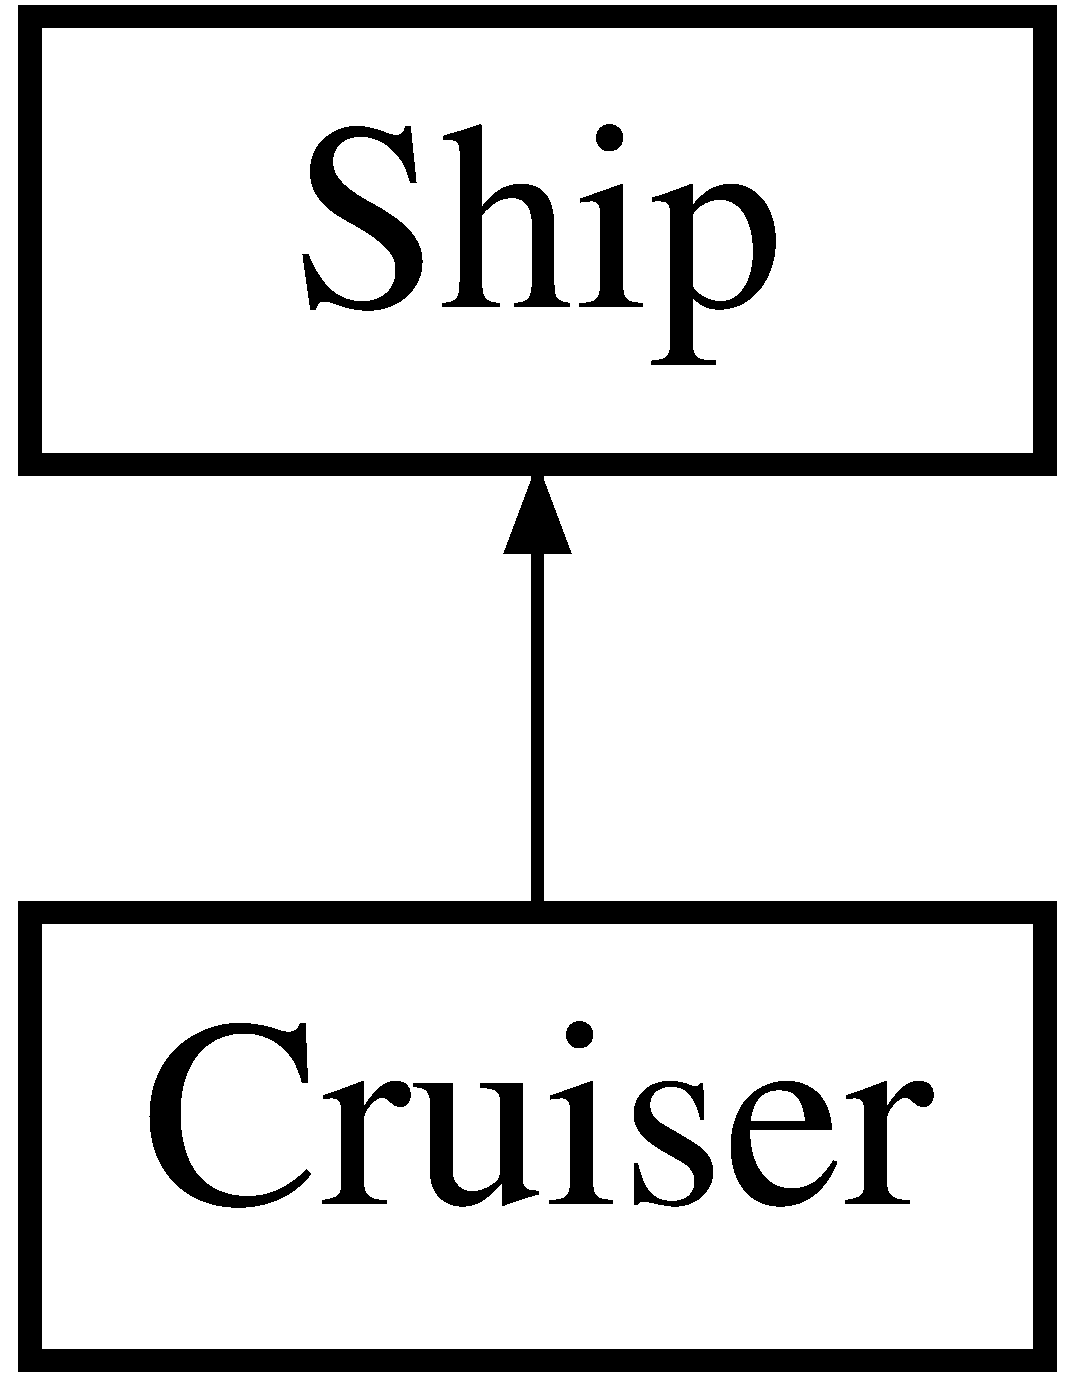
\includegraphics[height=2.000000cm]{class_cruiser}
\end{center}
\end{figure}
\subsection*{Public Member Functions}
\begin{DoxyCompactItemize}
\item 
\hyperlink{class_cruiser_a1b3e44174a2ee33c13d1d8a7ef69bf60}{Cruiser} (\hyperlink{struct_parameters}{Parameters} parameters\mbox{[}$\,$\mbox{]}, unsigned int i)
\item 
unsigned int \hyperlink{class_cruiser_a171a1c20f9eb95832cd19e2fb05cef6f}{number\+Of\+Squadrons} ()
\item 
virtual void \hyperlink{class_cruiser_aa61d6bff4f1a330dc1618ca3310792fe}{attack} ()
\end{DoxyCompactItemize}
\subsection*{Additional Inherited Members}


\subsection{Constructor \& Destructor Documentation}
\index{Cruiser@{Cruiser}!Cruiser@{Cruiser}}
\index{Cruiser@{Cruiser}!Cruiser@{Cruiser}}
\subsubsection[{\texorpdfstring{Cruiser(\+Parameters parameters[], unsigned int i)}{Cruiser(Parameters parameters[], unsigned int i)}}]{\setlength{\rightskip}{0pt plus 5cm}Cruiser\+::\+Cruiser (
\begin{DoxyParamCaption}
\item[{{\bf Parameters}}]{parameters\mbox{[}$\,$\mbox{]}, }
\item[{unsigned int}]{i}
\end{DoxyParamCaption}
)}\hypertarget{class_cruiser_a1b3e44174a2ee33c13d1d8a7ef69bf60}{}\label{class_cruiser_a1b3e44174a2ee33c13d1d8a7ef69bf60}


\subsection{Member Function Documentation}
\index{Cruiser@{Cruiser}!attack@{attack}}
\index{attack@{attack}!Cruiser@{Cruiser}}
\subsubsection[{\texorpdfstring{attack()}{attack()}}]{\setlength{\rightskip}{0pt plus 5cm}virtual void Cruiser\+::attack (
\begin{DoxyParamCaption}
{}
\end{DoxyParamCaption}
)\hspace{0.3cm}{\ttfamily [inline]}, {\ttfamily [virtual]}}\hypertarget{class_cruiser_aa61d6bff4f1a330dc1618ca3310792fe}{}\label{class_cruiser_aa61d6bff4f1a330dc1618ca3310792fe}


Implements \hyperlink{class_ship_a75d4d83e8f6bbaf06be9d1bf45c2bdd5}{Ship}.

\index{Cruiser@{Cruiser}!number\+Of\+Squadrons@{number\+Of\+Squadrons}}
\index{number\+Of\+Squadrons@{number\+Of\+Squadrons}!Cruiser@{Cruiser}}
\subsubsection[{\texorpdfstring{number\+Of\+Squadrons()}{numberOfSquadrons()}}]{\setlength{\rightskip}{0pt plus 5cm}unsigned int Cruiser\+::number\+Of\+Squadrons (
\begin{DoxyParamCaption}
{}
\end{DoxyParamCaption}
)\hspace{0.3cm}{\ttfamily [inline]}, {\ttfamily [virtual]}}\hypertarget{class_cruiser_a171a1c20f9eb95832cd19e2fb05cef6f}{}\label{class_cruiser_a171a1c20f9eb95832cd19e2fb05cef6f}


Implements \hyperlink{class_ship_abc3639e150f87a41a4ac1b770db7b56a}{Ship}.



The documentation for this class was generated from the following files\+:\begin{DoxyCompactItemize}
\item 
C\+:/\+Users/\+Piotr/\+Desktop/\+C\+Lion/proj\+\_\+naval\+\_\+battles/\hyperlink{_ship_8h}{Ship.\+h}\item 
C\+:/\+Users/\+Piotr/\+Desktop/\+C\+Lion/proj\+\_\+naval\+\_\+battles/\hyperlink{_ship_8cpp}{Ship.\+cpp}\end{DoxyCompactItemize}

\hypertarget{class_destroyer}{}\section{Destroyer Class Reference}
\label{class_destroyer}\index{Destroyer@{Destroyer}}


{\ttfamily \#include $<$Ship.\+h$>$}

Inheritance diagram for Destroyer\+:\begin{figure}[H]
\begin{center}
\leavevmode
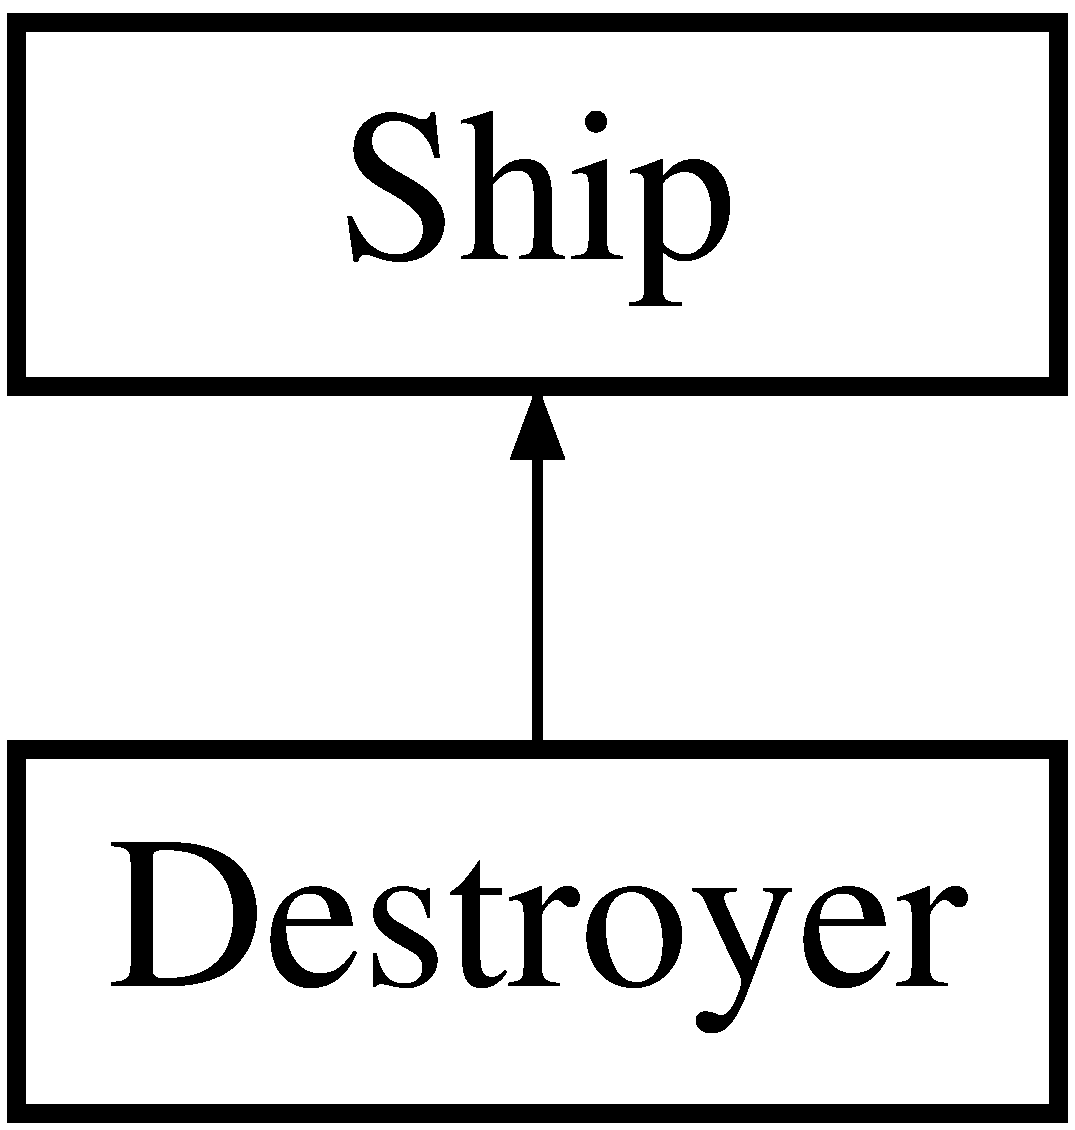
\includegraphics[height=2.000000cm]{class_destroyer}
\end{center}
\end{figure}
\subsection*{Public Member Functions}
\begin{DoxyCompactItemize}
\item 
\hyperlink{class_destroyer_ab39df898dcd1d4499fc79e424abf3675}{Destroyer} (\hyperlink{struct_parameters}{Parameters} parameters\mbox{[}$\,$\mbox{]}, unsigned int i)
\item 
unsigned int \hyperlink{class_destroyer_a6aa9dd38f320ba7eb65034b5e773be2c}{number\+Of\+Squadrons} ()
\item 
virtual void \hyperlink{class_destroyer_ab267533d886f2c64dbdb6af4365765f2}{attack} ()
\end{DoxyCompactItemize}
\subsection*{Additional Inherited Members}


\subsection{Constructor \& Destructor Documentation}
\index{Destroyer@{Destroyer}!Destroyer@{Destroyer}}
\index{Destroyer@{Destroyer}!Destroyer@{Destroyer}}
\subsubsection[{\texorpdfstring{Destroyer(\+Parameters parameters[], unsigned int i)}{Destroyer(Parameters parameters[], unsigned int i)}}]{\setlength{\rightskip}{0pt plus 5cm}Destroyer\+::\+Destroyer (
\begin{DoxyParamCaption}
\item[{{\bf Parameters}}]{parameters\mbox{[}$\,$\mbox{]}, }
\item[{unsigned int}]{i}
\end{DoxyParamCaption}
)}\hypertarget{class_destroyer_ab39df898dcd1d4499fc79e424abf3675}{}\label{class_destroyer_ab39df898dcd1d4499fc79e424abf3675}


\subsection{Member Function Documentation}
\index{Destroyer@{Destroyer}!attack@{attack}}
\index{attack@{attack}!Destroyer@{Destroyer}}
\subsubsection[{\texorpdfstring{attack()}{attack()}}]{\setlength{\rightskip}{0pt plus 5cm}virtual void Destroyer\+::attack (
\begin{DoxyParamCaption}
{}
\end{DoxyParamCaption}
)\hspace{0.3cm}{\ttfamily [inline]}, {\ttfamily [virtual]}}\hypertarget{class_destroyer_ab267533d886f2c64dbdb6af4365765f2}{}\label{class_destroyer_ab267533d886f2c64dbdb6af4365765f2}


Implements \hyperlink{class_ship_a75d4d83e8f6bbaf06be9d1bf45c2bdd5}{Ship}.

\index{Destroyer@{Destroyer}!number\+Of\+Squadrons@{number\+Of\+Squadrons}}
\index{number\+Of\+Squadrons@{number\+Of\+Squadrons}!Destroyer@{Destroyer}}
\subsubsection[{\texorpdfstring{number\+Of\+Squadrons()}{numberOfSquadrons()}}]{\setlength{\rightskip}{0pt plus 5cm}unsigned int Destroyer\+::number\+Of\+Squadrons (
\begin{DoxyParamCaption}
{}
\end{DoxyParamCaption}
)\hspace{0.3cm}{\ttfamily [inline]}, {\ttfamily [virtual]}}\hypertarget{class_destroyer_a6aa9dd38f320ba7eb65034b5e773be2c}{}\label{class_destroyer_a6aa9dd38f320ba7eb65034b5e773be2c}


Implements \hyperlink{class_ship_abc3639e150f87a41a4ac1b770db7b56a}{Ship}.



The documentation for this class was generated from the following files\+:\begin{DoxyCompactItemize}
\item 
C\+:/\+Users/\+Piotr/\+Desktop/\+C\+Lion/proj\+\_\+naval\+\_\+battles/\hyperlink{_ship_8h}{Ship.\+h}\item 
C\+:/\+Users/\+Piotr/\+Desktop/\+C\+Lion/proj\+\_\+naval\+\_\+battles/\hyperlink{_ship_8cpp}{Ship.\+cpp}\end{DoxyCompactItemize}

\hypertarget{struct_parameters}{}\section{Parameters Struct Reference}
\label{struct_parameters}\index{Parameters@{Parameters}}


{\ttfamily \#include $<$Functions.\+h$>$}

\subsection*{Public Attributes}
\begin{DoxyCompactItemize}
\item 
string \hyperlink{struct_parameters_a4b2f794128331583de50c0034c5998d2}{name}
\item 
\hyperlink{_functions_8h_ac7cd30cb79c1068579276e4cb287a2a7}{type\+Of\+Warship} \hyperlink{struct_parameters_a44a06370c5e94b66033e8f1178b90028}{type}
\item 
float \hyperlink{struct_parameters_a7bf937bc0aa16474d0146cf50ab4966c}{base\+Hp}
\item 
unsigned int \hyperlink{struct_parameters_a630c021422dbf1bdbbbacb269ed1a4fd}{armor}
\item 
double \hyperlink{struct_parameters_a7963432ebc43abe0bae0891dec48a987}{agility}
\item 
double \hyperlink{struct_parameters_ac2b1aba1f515ab5e2d253b5299736341}{camouflage}
\item 
double \hyperlink{struct_parameters_ade423be2e079e96d86a2b75cf5a1eb71}{chance\+For\+Arson}
\item 
unsigned int \hyperlink{struct_parameters_a7e763517fc70161d9edb3dd6290457bb}{amount\+Of\+Anti\+Aircraft\+Cannons}
\item 
unsigned int \hyperlink{struct_parameters_aba0a971e0cf5799f584ed4d00927aeea}{max\+Anti\+Aircraft\+Cannons\+Dmg}
\item 
unsigned int \hyperlink{struct_parameters_a13d11f0501e41cb7aa7bbb9757c5b5da}{amount\+Of\+Cannons}
\item 
unsigned int \hyperlink{struct_parameters_a8019e2c74fba6a925dde0364fa239a72}{max\+He\+Shell\+Dmg}
\item 
unsigned int \hyperlink{struct_parameters_ac1e0fe7e3177be12e7d4adcb9a3ceccd}{max\+Ap\+Shell\+Dmg}
\item 
unsigned int \hyperlink{struct_parameters_a025824e12728e624df3c4b85c57df3c4}{firing\+Range}
\item 
unsigned int \hyperlink{struct_parameters_a8665ae9bf926c6006625a1f95ee62fee}{chance\+For\+Arson\+By\+He}
\item 
unsigned int \hyperlink{struct_parameters_a53565b1bc98a61d79bd1f3c3b972e660}{amount\+Of\+Torpedos}
\item 
unsigned int \hyperlink{struct_parameters_a7c7434bba4d5209f8aa4d7c8ebcb8d64}{max\+Torpedo\+Dmg}
\item 
unsigned int \hyperlink{struct_parameters_aa0d7436c6b7ab9ec385fd13c6c957e58}{torpedo\+Range}
\item 
unsigned int \hyperlink{struct_parameters_a1217bb1ae5b1f5a5be2fbb91d1e27f33}{amount\+Of\+Squadrons}
\item 
unsigned int \hyperlink{struct_parameters_a827e9fb50cae3ec06d1fb3a5403e4975}{aircraft\+In\+Squadron}
\item 
unsigned int \hyperlink{struct_parameters_aeeafe82e2ab1457e0f8ecd7867e20022}{dmg\+Per\+Squadron}
\item 
float \hyperlink{struct_parameters_a17b4dc8d1fd6e19bef781d65d6578e83}{base\+Hp\+Per\+Squadron}
\end{DoxyCompactItemize}


\subsection{Member Data Documentation}
\index{Parameters@{Parameters}!agility@{agility}}
\index{agility@{agility}!Parameters@{Parameters}}
\subsubsection[{\texorpdfstring{agility}{agility}}]{\setlength{\rightskip}{0pt plus 5cm}double Parameters\+::agility}\hypertarget{struct_parameters_a7963432ebc43abe0bae0891dec48a987}{}\label{struct_parameters_a7963432ebc43abe0bae0891dec48a987}
\index{Parameters@{Parameters}!aircraft\+In\+Squadron@{aircraft\+In\+Squadron}}
\index{aircraft\+In\+Squadron@{aircraft\+In\+Squadron}!Parameters@{Parameters}}
\subsubsection[{\texorpdfstring{aircraft\+In\+Squadron}{aircraftInSquadron}}]{\setlength{\rightskip}{0pt plus 5cm}unsigned int Parameters\+::aircraft\+In\+Squadron}\hypertarget{struct_parameters_a827e9fb50cae3ec06d1fb3a5403e4975}{}\label{struct_parameters_a827e9fb50cae3ec06d1fb3a5403e4975}
\index{Parameters@{Parameters}!amount\+Of\+Anti\+Aircraft\+Cannons@{amount\+Of\+Anti\+Aircraft\+Cannons}}
\index{amount\+Of\+Anti\+Aircraft\+Cannons@{amount\+Of\+Anti\+Aircraft\+Cannons}!Parameters@{Parameters}}
\subsubsection[{\texorpdfstring{amount\+Of\+Anti\+Aircraft\+Cannons}{amountOfAntiAircraftCannons}}]{\setlength{\rightskip}{0pt plus 5cm}unsigned int Parameters\+::amount\+Of\+Anti\+Aircraft\+Cannons}\hypertarget{struct_parameters_a7e763517fc70161d9edb3dd6290457bb}{}\label{struct_parameters_a7e763517fc70161d9edb3dd6290457bb}
\index{Parameters@{Parameters}!amount\+Of\+Cannons@{amount\+Of\+Cannons}}
\index{amount\+Of\+Cannons@{amount\+Of\+Cannons}!Parameters@{Parameters}}
\subsubsection[{\texorpdfstring{amount\+Of\+Cannons}{amountOfCannons}}]{\setlength{\rightskip}{0pt plus 5cm}unsigned int Parameters\+::amount\+Of\+Cannons}\hypertarget{struct_parameters_a13d11f0501e41cb7aa7bbb9757c5b5da}{}\label{struct_parameters_a13d11f0501e41cb7aa7bbb9757c5b5da}
\index{Parameters@{Parameters}!amount\+Of\+Squadrons@{amount\+Of\+Squadrons}}
\index{amount\+Of\+Squadrons@{amount\+Of\+Squadrons}!Parameters@{Parameters}}
\subsubsection[{\texorpdfstring{amount\+Of\+Squadrons}{amountOfSquadrons}}]{\setlength{\rightskip}{0pt plus 5cm}unsigned int Parameters\+::amount\+Of\+Squadrons}\hypertarget{struct_parameters_a1217bb1ae5b1f5a5be2fbb91d1e27f33}{}\label{struct_parameters_a1217bb1ae5b1f5a5be2fbb91d1e27f33}
\index{Parameters@{Parameters}!amount\+Of\+Torpedos@{amount\+Of\+Torpedos}}
\index{amount\+Of\+Torpedos@{amount\+Of\+Torpedos}!Parameters@{Parameters}}
\subsubsection[{\texorpdfstring{amount\+Of\+Torpedos}{amountOfTorpedos}}]{\setlength{\rightskip}{0pt plus 5cm}unsigned int Parameters\+::amount\+Of\+Torpedos}\hypertarget{struct_parameters_a53565b1bc98a61d79bd1f3c3b972e660}{}\label{struct_parameters_a53565b1bc98a61d79bd1f3c3b972e660}
\index{Parameters@{Parameters}!armor@{armor}}
\index{armor@{armor}!Parameters@{Parameters}}
\subsubsection[{\texorpdfstring{armor}{armor}}]{\setlength{\rightskip}{0pt plus 5cm}unsigned int Parameters\+::armor}\hypertarget{struct_parameters_a630c021422dbf1bdbbbacb269ed1a4fd}{}\label{struct_parameters_a630c021422dbf1bdbbbacb269ed1a4fd}
\index{Parameters@{Parameters}!base\+Hp@{base\+Hp}}
\index{base\+Hp@{base\+Hp}!Parameters@{Parameters}}
\subsubsection[{\texorpdfstring{base\+Hp}{baseHp}}]{\setlength{\rightskip}{0pt plus 5cm}float Parameters\+::base\+Hp}\hypertarget{struct_parameters_a7bf937bc0aa16474d0146cf50ab4966c}{}\label{struct_parameters_a7bf937bc0aa16474d0146cf50ab4966c}
\index{Parameters@{Parameters}!base\+Hp\+Per\+Squadron@{base\+Hp\+Per\+Squadron}}
\index{base\+Hp\+Per\+Squadron@{base\+Hp\+Per\+Squadron}!Parameters@{Parameters}}
\subsubsection[{\texorpdfstring{base\+Hp\+Per\+Squadron}{baseHpPerSquadron}}]{\setlength{\rightskip}{0pt plus 5cm}float Parameters\+::base\+Hp\+Per\+Squadron}\hypertarget{struct_parameters_a17b4dc8d1fd6e19bef781d65d6578e83}{}\label{struct_parameters_a17b4dc8d1fd6e19bef781d65d6578e83}
\index{Parameters@{Parameters}!camouflage@{camouflage}}
\index{camouflage@{camouflage}!Parameters@{Parameters}}
\subsubsection[{\texorpdfstring{camouflage}{camouflage}}]{\setlength{\rightskip}{0pt plus 5cm}double Parameters\+::camouflage}\hypertarget{struct_parameters_ac2b1aba1f515ab5e2d253b5299736341}{}\label{struct_parameters_ac2b1aba1f515ab5e2d253b5299736341}
\index{Parameters@{Parameters}!chance\+For\+Arson@{chance\+For\+Arson}}
\index{chance\+For\+Arson@{chance\+For\+Arson}!Parameters@{Parameters}}
\subsubsection[{\texorpdfstring{chance\+For\+Arson}{chanceForArson}}]{\setlength{\rightskip}{0pt plus 5cm}double Parameters\+::chance\+For\+Arson}\hypertarget{struct_parameters_ade423be2e079e96d86a2b75cf5a1eb71}{}\label{struct_parameters_ade423be2e079e96d86a2b75cf5a1eb71}
\index{Parameters@{Parameters}!chance\+For\+Arson\+By\+He@{chance\+For\+Arson\+By\+He}}
\index{chance\+For\+Arson\+By\+He@{chance\+For\+Arson\+By\+He}!Parameters@{Parameters}}
\subsubsection[{\texorpdfstring{chance\+For\+Arson\+By\+He}{chanceForArsonByHe}}]{\setlength{\rightskip}{0pt plus 5cm}unsigned int Parameters\+::chance\+For\+Arson\+By\+He}\hypertarget{struct_parameters_a8665ae9bf926c6006625a1f95ee62fee}{}\label{struct_parameters_a8665ae9bf926c6006625a1f95ee62fee}
\index{Parameters@{Parameters}!dmg\+Per\+Squadron@{dmg\+Per\+Squadron}}
\index{dmg\+Per\+Squadron@{dmg\+Per\+Squadron}!Parameters@{Parameters}}
\subsubsection[{\texorpdfstring{dmg\+Per\+Squadron}{dmgPerSquadron}}]{\setlength{\rightskip}{0pt plus 5cm}unsigned int Parameters\+::dmg\+Per\+Squadron}\hypertarget{struct_parameters_aeeafe82e2ab1457e0f8ecd7867e20022}{}\label{struct_parameters_aeeafe82e2ab1457e0f8ecd7867e20022}
\index{Parameters@{Parameters}!firing\+Range@{firing\+Range}}
\index{firing\+Range@{firing\+Range}!Parameters@{Parameters}}
\subsubsection[{\texorpdfstring{firing\+Range}{firingRange}}]{\setlength{\rightskip}{0pt plus 5cm}unsigned int Parameters\+::firing\+Range}\hypertarget{struct_parameters_a025824e12728e624df3c4b85c57df3c4}{}\label{struct_parameters_a025824e12728e624df3c4b85c57df3c4}
\index{Parameters@{Parameters}!max\+Anti\+Aircraft\+Cannons\+Dmg@{max\+Anti\+Aircraft\+Cannons\+Dmg}}
\index{max\+Anti\+Aircraft\+Cannons\+Dmg@{max\+Anti\+Aircraft\+Cannons\+Dmg}!Parameters@{Parameters}}
\subsubsection[{\texorpdfstring{max\+Anti\+Aircraft\+Cannons\+Dmg}{maxAntiAircraftCannonsDmg}}]{\setlength{\rightskip}{0pt plus 5cm}unsigned int Parameters\+::max\+Anti\+Aircraft\+Cannons\+Dmg}\hypertarget{struct_parameters_aba0a971e0cf5799f584ed4d00927aeea}{}\label{struct_parameters_aba0a971e0cf5799f584ed4d00927aeea}
\index{Parameters@{Parameters}!max\+Ap\+Shell\+Dmg@{max\+Ap\+Shell\+Dmg}}
\index{max\+Ap\+Shell\+Dmg@{max\+Ap\+Shell\+Dmg}!Parameters@{Parameters}}
\subsubsection[{\texorpdfstring{max\+Ap\+Shell\+Dmg}{maxApShellDmg}}]{\setlength{\rightskip}{0pt plus 5cm}unsigned int Parameters\+::max\+Ap\+Shell\+Dmg}\hypertarget{struct_parameters_ac1e0fe7e3177be12e7d4adcb9a3ceccd}{}\label{struct_parameters_ac1e0fe7e3177be12e7d4adcb9a3ceccd}
\index{Parameters@{Parameters}!max\+He\+Shell\+Dmg@{max\+He\+Shell\+Dmg}}
\index{max\+He\+Shell\+Dmg@{max\+He\+Shell\+Dmg}!Parameters@{Parameters}}
\subsubsection[{\texorpdfstring{max\+He\+Shell\+Dmg}{maxHeShellDmg}}]{\setlength{\rightskip}{0pt plus 5cm}unsigned int Parameters\+::max\+He\+Shell\+Dmg}\hypertarget{struct_parameters_a8019e2c74fba6a925dde0364fa239a72}{}\label{struct_parameters_a8019e2c74fba6a925dde0364fa239a72}
\index{Parameters@{Parameters}!max\+Torpedo\+Dmg@{max\+Torpedo\+Dmg}}
\index{max\+Torpedo\+Dmg@{max\+Torpedo\+Dmg}!Parameters@{Parameters}}
\subsubsection[{\texorpdfstring{max\+Torpedo\+Dmg}{maxTorpedoDmg}}]{\setlength{\rightskip}{0pt plus 5cm}unsigned int Parameters\+::max\+Torpedo\+Dmg}\hypertarget{struct_parameters_a7c7434bba4d5209f8aa4d7c8ebcb8d64}{}\label{struct_parameters_a7c7434bba4d5209f8aa4d7c8ebcb8d64}
\index{Parameters@{Parameters}!name@{name}}
\index{name@{name}!Parameters@{Parameters}}
\subsubsection[{\texorpdfstring{name}{name}}]{\setlength{\rightskip}{0pt plus 5cm}string Parameters\+::name}\hypertarget{struct_parameters_a4b2f794128331583de50c0034c5998d2}{}\label{struct_parameters_a4b2f794128331583de50c0034c5998d2}
\index{Parameters@{Parameters}!torpedo\+Range@{torpedo\+Range}}
\index{torpedo\+Range@{torpedo\+Range}!Parameters@{Parameters}}
\subsubsection[{\texorpdfstring{torpedo\+Range}{torpedoRange}}]{\setlength{\rightskip}{0pt plus 5cm}unsigned int Parameters\+::torpedo\+Range}\hypertarget{struct_parameters_aa0d7436c6b7ab9ec385fd13c6c957e58}{}\label{struct_parameters_aa0d7436c6b7ab9ec385fd13c6c957e58}
\index{Parameters@{Parameters}!type@{type}}
\index{type@{type}!Parameters@{Parameters}}
\subsubsection[{\texorpdfstring{type}{type}}]{\setlength{\rightskip}{0pt plus 5cm}{\bf type\+Of\+Warship} Parameters\+::type}\hypertarget{struct_parameters_a44a06370c5e94b66033e8f1178b90028}{}\label{struct_parameters_a44a06370c5e94b66033e8f1178b90028}


The documentation for this struct was generated from the following file\+:\begin{DoxyCompactItemize}
\item 
C\+:/\+Users/\+Piotr/\+Desktop/\+C\+Lion/proj\+\_\+naval\+\_\+battles/\hyperlink{_functions_8h}{Functions.\+h}\end{DoxyCompactItemize}

\hypertarget{class_ship}{}\section{Ship Class Reference}
\label{class_ship}\index{Ship@{Ship}}


{\ttfamily \#include $<$Ship.\+h$>$}

Inheritance diagram for Ship\+:\begin{figure}[H]
\begin{center}
\leavevmode
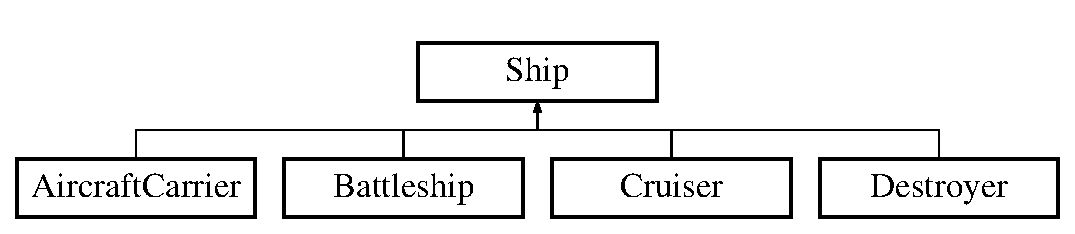
\includegraphics[height=2.000000cm]{class_ship}
\end{center}
\end{figure}
\subsection*{Public Member Functions}
\begin{DoxyCompactItemize}
\item 
void \hyperlink{class_ship_ae1a95dbd2102b3d6e7781fc9fae2d8eb}{Init} (\hyperlink{struct_parameters}{Parameters} parameters\mbox{[}$\,$\mbox{]}, unsigned int i)
\item 
bool \hyperlink{class_ship_a82c8b196cb492da2ea377dc9188a426f}{is\+Alive} ()
\item 
bool \hyperlink{class_ship_aa4c8a05e575b32f70d99220de9c864a1}{is\+Dead} ()
\item 
virtual void \hyperlink{class_ship_a75d4d83e8f6bbaf06be9d1bf45c2bdd5}{attack} ()=0
\item 
virtual unsigned int \hyperlink{class_ship_abc3639e150f87a41a4ac1b770db7b56a}{number\+Of\+Squadrons} ()=0
\item 
\hyperlink{_functions_8h_ac7cd30cb79c1068579276e4cb287a2a7}{type\+Of\+Warship} \hyperlink{class_ship_a6636075f5ef1f6a2e0503f5ab370aead}{what\+Type} ()
\item 
void \hyperlink{class_ship_a8132d27eb12189d50da3c3eafdf159b5}{description} (\hyperlink{class_ship}{Ship} $\ast$wsk1, \hyperlink{class_ship}{Ship} $\ast$wsk2)
\end{DoxyCompactItemize}
\subsection*{Protected Attributes}
\begin{DoxyCompactItemize}
\item 
string \hyperlink{class_ship_a68cf161799aadcbbe1c7b28b9dd10849}{\+\_\+name}
\item 
\hyperlink{_functions_8h_ac7cd30cb79c1068579276e4cb287a2a7}{type\+Of\+Warship} \hyperlink{class_ship_a5a32460ba76649a09aa9c9d4df332217}{\+\_\+type}
\item 
float \hyperlink{class_ship_af95a5ee3b4f3ffc4ab069a5dce7baa16}{base\+Hp}
\item 
float \hyperlink{class_ship_a2651d11a4926fe1b2eb65883565e8bd3}{\+\_\+hp}
\item 
unsigned int \hyperlink{class_ship_ac47a2f3ff405ca582bb0eb40c656c0e3}{\+\_\+armor}
\item 
double \hyperlink{class_ship_a28defb88168c7f977ae06a023a2de772}{\+\_\+agility}
\item 
double \hyperlink{class_ship_aa0df6c32a4745b65ba7bb0ed4368f15e}{\+\_\+camouflage}
\item 
double \hyperlink{class_ship_ae77c4ff11f205f30804f750e36a956ab}{\+\_\+chance\+For\+Arson}
\item 
unsigned int \hyperlink{class_ship_a347e40d66fe5a0282309ffd280d5f596}{\+\_\+amount\+Of\+Cannons}
\item 
unsigned int \hyperlink{class_ship_ab24d3443c476283386c89754fd433670}{\+\_\+max\+He\+Shell\+Dmg}
\item 
unsigned int \hyperlink{class_ship_aa936c394b1cc8f19cb4e5d66a7223e63}{\+\_\+max\+Ap\+Shell\+Dmg}
\item 
unsigned int \hyperlink{class_ship_a070c1763b821ed7ba50931558283e82c}{\+\_\+firing\+Range}
\item 
unsigned int \hyperlink{class_ship_a5ae7f8df8dec0c92ce8f778e37c0fafb}{\+\_\+chance\+For\+Arson\+By\+He}
\item 
unsigned int \hyperlink{class_ship_ac6b6499ae6b669db54cbd640e9bba7ec}{\+\_\+amount\+Of\+Anti\+Aircraft\+Cannons}
\item 
unsigned int \hyperlink{class_ship_a30a5533d9feec6fea05ae3b9472361b6}{\+\_\+max\+Anti\+Aircraft\+Cannons\+Dmg}
\item 
unsigned int \hyperlink{class_ship_aeb1a24d770dc9dc85c5b4a70bf5bbff5}{\+\_\+amount\+Of\+Torpedos}
\item 
unsigned int \hyperlink{class_ship_adc1f7e5d7b3db9420ce78c81ba7d64f1}{\+\_\+max\+Torpedo\+Dmg}
\item 
unsigned int \hyperlink{class_ship_af3e30d448490de75365944a9b8715445}{\+\_\+torpedo\+Range}
\item 
unsigned int \hyperlink{class_ship_a6177a736c0cefe335b0aa4ea5fe59958}{\+\_\+amount\+Of\+Squadrons}
\item 
unsigned int \hyperlink{class_ship_a2c837b0bd540df9da7826ee0e2ac0bf1}{\+\_\+aircraft\+In\+Squadron}
\item 
unsigned int \hyperlink{class_ship_a73bfeb8252997fc26bfb0c994ec1c0df}{\+\_\+dmg\+Per\+Squadron}
\item 
float \hyperlink{class_ship_a648d4df59880f64ee8f7d1b30dc7c3f2}{\+\_\+base\+Hp\+Per\+Squadron}
\end{DoxyCompactItemize}
\subsection*{Friends}
\begin{DoxyCompactItemize}
\item 
void \hyperlink{class_ship_ac66ecfb017374d98a9930670ec1c8945}{make\+Dead} (\hyperlink{class_ship}{Ship} $\ast$wsk)
\item 
int \hyperlink{class_ship_accbeca51df41fe5d3068313403c14223}{war} (\hyperlink{class_ship}{Ship} $\ast$wsk1, \hyperlink{class_ship}{Ship} $\ast$wsk2)
\end{DoxyCompactItemize}


\subsection{Member Function Documentation}
\index{Ship@{Ship}!attack@{attack}}
\index{attack@{attack}!Ship@{Ship}}
\subsubsection[{\texorpdfstring{attack()=0}{attack()=0}}]{\setlength{\rightskip}{0pt plus 5cm}virtual void Ship\+::attack (
\begin{DoxyParamCaption}
{}
\end{DoxyParamCaption}
)\hspace{0.3cm}{\ttfamily [pure virtual]}}\hypertarget{class_ship_a75d4d83e8f6bbaf06be9d1bf45c2bdd5}{}\label{class_ship_a75d4d83e8f6bbaf06be9d1bf45c2bdd5}


Implemented in \hyperlink{class_aircraft_carrier_a6a4f9376d570301e2a720d699d61af1c}{Aircraft\+Carrier}, \hyperlink{class_battleship_a599cd8efe7d763b170b1352813cf47f1}{Battleship}, \hyperlink{class_cruiser_aa61d6bff4f1a330dc1618ca3310792fe}{Cruiser}, and \hyperlink{class_destroyer_ab267533d886f2c64dbdb6af4365765f2}{Destroyer}.

\index{Ship@{Ship}!description@{description}}
\index{description@{description}!Ship@{Ship}}
\subsubsection[{\texorpdfstring{description(\+Ship $\ast$wsk1, Ship $\ast$wsk2)}{description(Ship *wsk1, Ship *wsk2)}}]{\setlength{\rightskip}{0pt plus 5cm}void Ship\+::description (
\begin{DoxyParamCaption}
\item[{{\bf Ship} $\ast$}]{wsk1, }
\item[{{\bf Ship} $\ast$}]{wsk2}
\end{DoxyParamCaption}
)}\hypertarget{class_ship_a8132d27eb12189d50da3c3eafdf159b5}{}\label{class_ship_a8132d27eb12189d50da3c3eafdf159b5}
\index{Ship@{Ship}!Init@{Init}}
\index{Init@{Init}!Ship@{Ship}}
\subsubsection[{\texorpdfstring{Init(\+Parameters parameters[], unsigned int i)}{Init(Parameters parameters[], unsigned int i)}}]{\setlength{\rightskip}{0pt plus 5cm}void Ship\+::\+Init (
\begin{DoxyParamCaption}
\item[{{\bf Parameters}}]{parameters\mbox{[}$\,$\mbox{]}, }
\item[{unsigned int}]{i}
\end{DoxyParamCaption}
)}\hypertarget{class_ship_ae1a95dbd2102b3d6e7781fc9fae2d8eb}{}\label{class_ship_ae1a95dbd2102b3d6e7781fc9fae2d8eb}
\index{Ship@{Ship}!is\+Alive@{is\+Alive}}
\index{is\+Alive@{is\+Alive}!Ship@{Ship}}
\subsubsection[{\texorpdfstring{is\+Alive()}{isAlive()}}]{\setlength{\rightskip}{0pt plus 5cm}bool Ship\+::is\+Alive (
\begin{DoxyParamCaption}
{}
\end{DoxyParamCaption}
)}\hypertarget{class_ship_a82c8b196cb492da2ea377dc9188a426f}{}\label{class_ship_a82c8b196cb492da2ea377dc9188a426f}
\index{Ship@{Ship}!is\+Dead@{is\+Dead}}
\index{is\+Dead@{is\+Dead}!Ship@{Ship}}
\subsubsection[{\texorpdfstring{is\+Dead()}{isDead()}}]{\setlength{\rightskip}{0pt plus 5cm}bool Ship\+::is\+Dead (
\begin{DoxyParamCaption}
{}
\end{DoxyParamCaption}
)}\hypertarget{class_ship_aa4c8a05e575b32f70d99220de9c864a1}{}\label{class_ship_aa4c8a05e575b32f70d99220de9c864a1}
\index{Ship@{Ship}!number\+Of\+Squadrons@{number\+Of\+Squadrons}}
\index{number\+Of\+Squadrons@{number\+Of\+Squadrons}!Ship@{Ship}}
\subsubsection[{\texorpdfstring{number\+Of\+Squadrons()=0}{numberOfSquadrons()=0}}]{\setlength{\rightskip}{0pt plus 5cm}virtual unsigned int Ship\+::number\+Of\+Squadrons (
\begin{DoxyParamCaption}
{}
\end{DoxyParamCaption}
)\hspace{0.3cm}{\ttfamily [pure virtual]}}\hypertarget{class_ship_abc3639e150f87a41a4ac1b770db7b56a}{}\label{class_ship_abc3639e150f87a41a4ac1b770db7b56a}


Implemented in \hyperlink{class_aircraft_carrier_a1521dc1e79308c4ebd1b979a48878446}{Aircraft\+Carrier}, \hyperlink{class_battleship_af64957b1b5dbc5c0fab74c90b94de9d0}{Battleship}, \hyperlink{class_cruiser_a171a1c20f9eb95832cd19e2fb05cef6f}{Cruiser}, and \hyperlink{class_destroyer_a6aa9dd38f320ba7eb65034b5e773be2c}{Destroyer}.

\index{Ship@{Ship}!what\+Type@{what\+Type}}
\index{what\+Type@{what\+Type}!Ship@{Ship}}
\subsubsection[{\texorpdfstring{what\+Type()}{whatType()}}]{\setlength{\rightskip}{0pt plus 5cm}{\bf type\+Of\+Warship} Ship\+::what\+Type (
\begin{DoxyParamCaption}
{}
\end{DoxyParamCaption}
)\hspace{0.3cm}{\ttfamily [inline]}}\hypertarget{class_ship_a6636075f5ef1f6a2e0503f5ab370aead}{}\label{class_ship_a6636075f5ef1f6a2e0503f5ab370aead}


\subsection{Friends And Related Function Documentation}
\index{Ship@{Ship}!make\+Dead@{make\+Dead}}
\index{make\+Dead@{make\+Dead}!Ship@{Ship}}
\subsubsection[{\texorpdfstring{make\+Dead}{makeDead}}]{\setlength{\rightskip}{0pt plus 5cm}void make\+Dead (
\begin{DoxyParamCaption}
\item[{{\bf Ship} $\ast$}]{wsk}
\end{DoxyParamCaption}
)\hspace{0.3cm}{\ttfamily [friend]}}\hypertarget{class_ship_ac66ecfb017374d98a9930670ec1c8945}{}\label{class_ship_ac66ecfb017374d98a9930670ec1c8945}
\index{Ship@{Ship}!war@{war}}
\index{war@{war}!Ship@{Ship}}
\subsubsection[{\texorpdfstring{war}{war}}]{\setlength{\rightskip}{0pt plus 5cm}int war (
\begin{DoxyParamCaption}
\item[{{\bf Ship} $\ast$}]{wsk1, }
\item[{{\bf Ship} $\ast$}]{wsk2}
\end{DoxyParamCaption}
)\hspace{0.3cm}{\ttfamily [friend]}}\hypertarget{class_ship_accbeca51df41fe5d3068313403c14223}{}\label{class_ship_accbeca51df41fe5d3068313403c14223}


\subsection{Member Data Documentation}
\index{Ship@{Ship}!\+\_\+agility@{\+\_\+agility}}
\index{\+\_\+agility@{\+\_\+agility}!Ship@{Ship}}
\subsubsection[{\texorpdfstring{\+\_\+agility}{_agility}}]{\setlength{\rightskip}{0pt plus 5cm}double Ship\+::\+\_\+agility\hspace{0.3cm}{\ttfamily [protected]}}\hypertarget{class_ship_a28defb88168c7f977ae06a023a2de772}{}\label{class_ship_a28defb88168c7f977ae06a023a2de772}
\index{Ship@{Ship}!\+\_\+aircraft\+In\+Squadron@{\+\_\+aircraft\+In\+Squadron}}
\index{\+\_\+aircraft\+In\+Squadron@{\+\_\+aircraft\+In\+Squadron}!Ship@{Ship}}
\subsubsection[{\texorpdfstring{\+\_\+aircraft\+In\+Squadron}{_aircraftInSquadron}}]{\setlength{\rightskip}{0pt plus 5cm}unsigned int Ship\+::\+\_\+aircraft\+In\+Squadron\hspace{0.3cm}{\ttfamily [protected]}}\hypertarget{class_ship_a2c837b0bd540df9da7826ee0e2ac0bf1}{}\label{class_ship_a2c837b0bd540df9da7826ee0e2ac0bf1}
\index{Ship@{Ship}!\+\_\+amount\+Of\+Anti\+Aircraft\+Cannons@{\+\_\+amount\+Of\+Anti\+Aircraft\+Cannons}}
\index{\+\_\+amount\+Of\+Anti\+Aircraft\+Cannons@{\+\_\+amount\+Of\+Anti\+Aircraft\+Cannons}!Ship@{Ship}}
\subsubsection[{\texorpdfstring{\+\_\+amount\+Of\+Anti\+Aircraft\+Cannons}{_amountOfAntiAircraftCannons}}]{\setlength{\rightskip}{0pt plus 5cm}unsigned int Ship\+::\+\_\+amount\+Of\+Anti\+Aircraft\+Cannons\hspace{0.3cm}{\ttfamily [protected]}}\hypertarget{class_ship_ac6b6499ae6b669db54cbd640e9bba7ec}{}\label{class_ship_ac6b6499ae6b669db54cbd640e9bba7ec}
\index{Ship@{Ship}!\+\_\+amount\+Of\+Cannons@{\+\_\+amount\+Of\+Cannons}}
\index{\+\_\+amount\+Of\+Cannons@{\+\_\+amount\+Of\+Cannons}!Ship@{Ship}}
\subsubsection[{\texorpdfstring{\+\_\+amount\+Of\+Cannons}{_amountOfCannons}}]{\setlength{\rightskip}{0pt plus 5cm}unsigned int Ship\+::\+\_\+amount\+Of\+Cannons\hspace{0.3cm}{\ttfamily [protected]}}\hypertarget{class_ship_a347e40d66fe5a0282309ffd280d5f596}{}\label{class_ship_a347e40d66fe5a0282309ffd280d5f596}
\index{Ship@{Ship}!\+\_\+amount\+Of\+Squadrons@{\+\_\+amount\+Of\+Squadrons}}
\index{\+\_\+amount\+Of\+Squadrons@{\+\_\+amount\+Of\+Squadrons}!Ship@{Ship}}
\subsubsection[{\texorpdfstring{\+\_\+amount\+Of\+Squadrons}{_amountOfSquadrons}}]{\setlength{\rightskip}{0pt plus 5cm}unsigned int Ship\+::\+\_\+amount\+Of\+Squadrons\hspace{0.3cm}{\ttfamily [protected]}}\hypertarget{class_ship_a6177a736c0cefe335b0aa4ea5fe59958}{}\label{class_ship_a6177a736c0cefe335b0aa4ea5fe59958}
\index{Ship@{Ship}!\+\_\+amount\+Of\+Torpedos@{\+\_\+amount\+Of\+Torpedos}}
\index{\+\_\+amount\+Of\+Torpedos@{\+\_\+amount\+Of\+Torpedos}!Ship@{Ship}}
\subsubsection[{\texorpdfstring{\+\_\+amount\+Of\+Torpedos}{_amountOfTorpedos}}]{\setlength{\rightskip}{0pt plus 5cm}unsigned int Ship\+::\+\_\+amount\+Of\+Torpedos\hspace{0.3cm}{\ttfamily [protected]}}\hypertarget{class_ship_aeb1a24d770dc9dc85c5b4a70bf5bbff5}{}\label{class_ship_aeb1a24d770dc9dc85c5b4a70bf5bbff5}
\index{Ship@{Ship}!\+\_\+armor@{\+\_\+armor}}
\index{\+\_\+armor@{\+\_\+armor}!Ship@{Ship}}
\subsubsection[{\texorpdfstring{\+\_\+armor}{_armor}}]{\setlength{\rightskip}{0pt plus 5cm}unsigned int Ship\+::\+\_\+armor\hspace{0.3cm}{\ttfamily [protected]}}\hypertarget{class_ship_ac47a2f3ff405ca582bb0eb40c656c0e3}{}\label{class_ship_ac47a2f3ff405ca582bb0eb40c656c0e3}
\index{Ship@{Ship}!\+\_\+base\+Hp\+Per\+Squadron@{\+\_\+base\+Hp\+Per\+Squadron}}
\index{\+\_\+base\+Hp\+Per\+Squadron@{\+\_\+base\+Hp\+Per\+Squadron}!Ship@{Ship}}
\subsubsection[{\texorpdfstring{\+\_\+base\+Hp\+Per\+Squadron}{_baseHpPerSquadron}}]{\setlength{\rightskip}{0pt plus 5cm}float Ship\+::\+\_\+base\+Hp\+Per\+Squadron\hspace{0.3cm}{\ttfamily [protected]}}\hypertarget{class_ship_a648d4df59880f64ee8f7d1b30dc7c3f2}{}\label{class_ship_a648d4df59880f64ee8f7d1b30dc7c3f2}
\index{Ship@{Ship}!\+\_\+camouflage@{\+\_\+camouflage}}
\index{\+\_\+camouflage@{\+\_\+camouflage}!Ship@{Ship}}
\subsubsection[{\texorpdfstring{\+\_\+camouflage}{_camouflage}}]{\setlength{\rightskip}{0pt plus 5cm}double Ship\+::\+\_\+camouflage\hspace{0.3cm}{\ttfamily [protected]}}\hypertarget{class_ship_aa0df6c32a4745b65ba7bb0ed4368f15e}{}\label{class_ship_aa0df6c32a4745b65ba7bb0ed4368f15e}
\index{Ship@{Ship}!\+\_\+chance\+For\+Arson@{\+\_\+chance\+For\+Arson}}
\index{\+\_\+chance\+For\+Arson@{\+\_\+chance\+For\+Arson}!Ship@{Ship}}
\subsubsection[{\texorpdfstring{\+\_\+chance\+For\+Arson}{_chanceForArson}}]{\setlength{\rightskip}{0pt plus 5cm}double Ship\+::\+\_\+chance\+For\+Arson\hspace{0.3cm}{\ttfamily [protected]}}\hypertarget{class_ship_ae77c4ff11f205f30804f750e36a956ab}{}\label{class_ship_ae77c4ff11f205f30804f750e36a956ab}
\index{Ship@{Ship}!\+\_\+chance\+For\+Arson\+By\+He@{\+\_\+chance\+For\+Arson\+By\+He}}
\index{\+\_\+chance\+For\+Arson\+By\+He@{\+\_\+chance\+For\+Arson\+By\+He}!Ship@{Ship}}
\subsubsection[{\texorpdfstring{\+\_\+chance\+For\+Arson\+By\+He}{_chanceForArsonByHe}}]{\setlength{\rightskip}{0pt plus 5cm}unsigned int Ship\+::\+\_\+chance\+For\+Arson\+By\+He\hspace{0.3cm}{\ttfamily [protected]}}\hypertarget{class_ship_a5ae7f8df8dec0c92ce8f778e37c0fafb}{}\label{class_ship_a5ae7f8df8dec0c92ce8f778e37c0fafb}
\index{Ship@{Ship}!\+\_\+dmg\+Per\+Squadron@{\+\_\+dmg\+Per\+Squadron}}
\index{\+\_\+dmg\+Per\+Squadron@{\+\_\+dmg\+Per\+Squadron}!Ship@{Ship}}
\subsubsection[{\texorpdfstring{\+\_\+dmg\+Per\+Squadron}{_dmgPerSquadron}}]{\setlength{\rightskip}{0pt plus 5cm}unsigned int Ship\+::\+\_\+dmg\+Per\+Squadron\hspace{0.3cm}{\ttfamily [protected]}}\hypertarget{class_ship_a73bfeb8252997fc26bfb0c994ec1c0df}{}\label{class_ship_a73bfeb8252997fc26bfb0c994ec1c0df}
\index{Ship@{Ship}!\+\_\+firing\+Range@{\+\_\+firing\+Range}}
\index{\+\_\+firing\+Range@{\+\_\+firing\+Range}!Ship@{Ship}}
\subsubsection[{\texorpdfstring{\+\_\+firing\+Range}{_firingRange}}]{\setlength{\rightskip}{0pt plus 5cm}unsigned int Ship\+::\+\_\+firing\+Range\hspace{0.3cm}{\ttfamily [protected]}}\hypertarget{class_ship_a070c1763b821ed7ba50931558283e82c}{}\label{class_ship_a070c1763b821ed7ba50931558283e82c}
\index{Ship@{Ship}!\+\_\+hp@{\+\_\+hp}}
\index{\+\_\+hp@{\+\_\+hp}!Ship@{Ship}}
\subsubsection[{\texorpdfstring{\+\_\+hp}{_hp}}]{\setlength{\rightskip}{0pt plus 5cm}float Ship\+::\+\_\+hp\hspace{0.3cm}{\ttfamily [protected]}}\hypertarget{class_ship_a2651d11a4926fe1b2eb65883565e8bd3}{}\label{class_ship_a2651d11a4926fe1b2eb65883565e8bd3}
\index{Ship@{Ship}!\+\_\+max\+Anti\+Aircraft\+Cannons\+Dmg@{\+\_\+max\+Anti\+Aircraft\+Cannons\+Dmg}}
\index{\+\_\+max\+Anti\+Aircraft\+Cannons\+Dmg@{\+\_\+max\+Anti\+Aircraft\+Cannons\+Dmg}!Ship@{Ship}}
\subsubsection[{\texorpdfstring{\+\_\+max\+Anti\+Aircraft\+Cannons\+Dmg}{_maxAntiAircraftCannonsDmg}}]{\setlength{\rightskip}{0pt plus 5cm}unsigned int Ship\+::\+\_\+max\+Anti\+Aircraft\+Cannons\+Dmg\hspace{0.3cm}{\ttfamily [protected]}}\hypertarget{class_ship_a30a5533d9feec6fea05ae3b9472361b6}{}\label{class_ship_a30a5533d9feec6fea05ae3b9472361b6}
\index{Ship@{Ship}!\+\_\+max\+Ap\+Shell\+Dmg@{\+\_\+max\+Ap\+Shell\+Dmg}}
\index{\+\_\+max\+Ap\+Shell\+Dmg@{\+\_\+max\+Ap\+Shell\+Dmg}!Ship@{Ship}}
\subsubsection[{\texorpdfstring{\+\_\+max\+Ap\+Shell\+Dmg}{_maxApShellDmg}}]{\setlength{\rightskip}{0pt plus 5cm}unsigned int Ship\+::\+\_\+max\+Ap\+Shell\+Dmg\hspace{0.3cm}{\ttfamily [protected]}}\hypertarget{class_ship_aa936c394b1cc8f19cb4e5d66a7223e63}{}\label{class_ship_aa936c394b1cc8f19cb4e5d66a7223e63}
\index{Ship@{Ship}!\+\_\+max\+He\+Shell\+Dmg@{\+\_\+max\+He\+Shell\+Dmg}}
\index{\+\_\+max\+He\+Shell\+Dmg@{\+\_\+max\+He\+Shell\+Dmg}!Ship@{Ship}}
\subsubsection[{\texorpdfstring{\+\_\+max\+He\+Shell\+Dmg}{_maxHeShellDmg}}]{\setlength{\rightskip}{0pt plus 5cm}unsigned int Ship\+::\+\_\+max\+He\+Shell\+Dmg\hspace{0.3cm}{\ttfamily [protected]}}\hypertarget{class_ship_ab24d3443c476283386c89754fd433670}{}\label{class_ship_ab24d3443c476283386c89754fd433670}
\index{Ship@{Ship}!\+\_\+max\+Torpedo\+Dmg@{\+\_\+max\+Torpedo\+Dmg}}
\index{\+\_\+max\+Torpedo\+Dmg@{\+\_\+max\+Torpedo\+Dmg}!Ship@{Ship}}
\subsubsection[{\texorpdfstring{\+\_\+max\+Torpedo\+Dmg}{_maxTorpedoDmg}}]{\setlength{\rightskip}{0pt plus 5cm}unsigned int Ship\+::\+\_\+max\+Torpedo\+Dmg\hspace{0.3cm}{\ttfamily [protected]}}\hypertarget{class_ship_adc1f7e5d7b3db9420ce78c81ba7d64f1}{}\label{class_ship_adc1f7e5d7b3db9420ce78c81ba7d64f1}
\index{Ship@{Ship}!\+\_\+name@{\+\_\+name}}
\index{\+\_\+name@{\+\_\+name}!Ship@{Ship}}
\subsubsection[{\texorpdfstring{\+\_\+name}{_name}}]{\setlength{\rightskip}{0pt plus 5cm}string Ship\+::\+\_\+name\hspace{0.3cm}{\ttfamily [protected]}}\hypertarget{class_ship_a68cf161799aadcbbe1c7b28b9dd10849}{}\label{class_ship_a68cf161799aadcbbe1c7b28b9dd10849}
\index{Ship@{Ship}!\+\_\+torpedo\+Range@{\+\_\+torpedo\+Range}}
\index{\+\_\+torpedo\+Range@{\+\_\+torpedo\+Range}!Ship@{Ship}}
\subsubsection[{\texorpdfstring{\+\_\+torpedo\+Range}{_torpedoRange}}]{\setlength{\rightskip}{0pt plus 5cm}unsigned int Ship\+::\+\_\+torpedo\+Range\hspace{0.3cm}{\ttfamily [protected]}}\hypertarget{class_ship_af3e30d448490de75365944a9b8715445}{}\label{class_ship_af3e30d448490de75365944a9b8715445}
\index{Ship@{Ship}!\+\_\+type@{\+\_\+type}}
\index{\+\_\+type@{\+\_\+type}!Ship@{Ship}}
\subsubsection[{\texorpdfstring{\+\_\+type}{_type}}]{\setlength{\rightskip}{0pt plus 5cm}{\bf type\+Of\+Warship} Ship\+::\+\_\+type\hspace{0.3cm}{\ttfamily [protected]}}\hypertarget{class_ship_a5a32460ba76649a09aa9c9d4df332217}{}\label{class_ship_a5a32460ba76649a09aa9c9d4df332217}
\index{Ship@{Ship}!base\+Hp@{base\+Hp}}
\index{base\+Hp@{base\+Hp}!Ship@{Ship}}
\subsubsection[{\texorpdfstring{base\+Hp}{baseHp}}]{\setlength{\rightskip}{0pt plus 5cm}float Ship\+::base\+Hp\hspace{0.3cm}{\ttfamily [protected]}}\hypertarget{class_ship_af95a5ee3b4f3ffc4ab069a5dce7baa16}{}\label{class_ship_af95a5ee3b4f3ffc4ab069a5dce7baa16}


The documentation for this class was generated from the following files\+:\begin{DoxyCompactItemize}
\item 
C\+:/\+Users/\+Piotr/\+Desktop/\+C\+Lion/proj\+\_\+naval\+\_\+battles/\hyperlink{_ship_8h}{Ship.\+h}\item 
C\+:/\+Users/\+Piotr/\+Desktop/\+C\+Lion/proj\+\_\+naval\+\_\+battles/\hyperlink{_ship_8cpp}{Ship.\+cpp}\end{DoxyCompactItemize}

\hypertarget{structsite}{}\section{site Struct Reference}
\label{structsite}\index{site@{site}}


{\ttfamily \#include $<$Battle.\+h$>$}

\subsection*{Public Attributes}
\begin{DoxyCompactItemize}
\item 
string \hyperlink{structsite_ae4192402457d29b056ec34ebc57b535e}{site\+Name}
\item 
vector$<$ \hyperlink{class_destroyer}{Destroyer} $>$ \hyperlink{structsite_af920c7e8cfc6306cde0d45b9850af20e}{\+\_\+destroyers}
\item 
vector$<$ \hyperlink{class_cruiser}{Cruiser} $>$ \hyperlink{structsite_ae2ae4dc2c4f396ead27233eb03e7756f}{\+\_\+cruisers}
\item 
vector$<$ \hyperlink{class_battleship}{Battleship} $>$ \hyperlink{structsite_ad15b3351029ffbb3ea21c75e05f6a1b3}{\+\_\+battleships}
\item 
vector$<$ \hyperlink{class_aircraft_carrier}{Aircraft\+Carrier} $>$ \hyperlink{structsite_a19551d075f273b4c5546f704f01ad471}{\+\_\+aircraft\+Carriers}
\end{DoxyCompactItemize}


\subsection{Member Data Documentation}
\index{site@{site}!\+\_\+aircraft\+Carriers@{\+\_\+aircraft\+Carriers}}
\index{\+\_\+aircraft\+Carriers@{\+\_\+aircraft\+Carriers}!site@{site}}
\subsubsection[{\texorpdfstring{\+\_\+aircraft\+Carriers}{_aircraftCarriers}}]{\setlength{\rightskip}{0pt plus 5cm}vector$<${\bf Aircraft\+Carrier}$>$ site\+::\+\_\+aircraft\+Carriers}\hypertarget{structsite_a19551d075f273b4c5546f704f01ad471}{}\label{structsite_a19551d075f273b4c5546f704f01ad471}
\index{site@{site}!\+\_\+battleships@{\+\_\+battleships}}
\index{\+\_\+battleships@{\+\_\+battleships}!site@{site}}
\subsubsection[{\texorpdfstring{\+\_\+battleships}{_battleships}}]{\setlength{\rightskip}{0pt plus 5cm}vector$<${\bf Battleship}$>$ site\+::\+\_\+battleships}\hypertarget{structsite_ad15b3351029ffbb3ea21c75e05f6a1b3}{}\label{structsite_ad15b3351029ffbb3ea21c75e05f6a1b3}
\index{site@{site}!\+\_\+cruisers@{\+\_\+cruisers}}
\index{\+\_\+cruisers@{\+\_\+cruisers}!site@{site}}
\subsubsection[{\texorpdfstring{\+\_\+cruisers}{_cruisers}}]{\setlength{\rightskip}{0pt plus 5cm}vector$<${\bf Cruiser}$>$ site\+::\+\_\+cruisers}\hypertarget{structsite_ae2ae4dc2c4f396ead27233eb03e7756f}{}\label{structsite_ae2ae4dc2c4f396ead27233eb03e7756f}
\index{site@{site}!\+\_\+destroyers@{\+\_\+destroyers}}
\index{\+\_\+destroyers@{\+\_\+destroyers}!site@{site}}
\subsubsection[{\texorpdfstring{\+\_\+destroyers}{_destroyers}}]{\setlength{\rightskip}{0pt plus 5cm}vector$<${\bf Destroyer}$>$ site\+::\+\_\+destroyers}\hypertarget{structsite_af920c7e8cfc6306cde0d45b9850af20e}{}\label{structsite_af920c7e8cfc6306cde0d45b9850af20e}
\index{site@{site}!site\+Name@{site\+Name}}
\index{site\+Name@{site\+Name}!site@{site}}
\subsubsection[{\texorpdfstring{site\+Name}{siteName}}]{\setlength{\rightskip}{0pt plus 5cm}string site\+::site\+Name}\hypertarget{structsite_ae4192402457d29b056ec34ebc57b535e}{}\label{structsite_ae4192402457d29b056ec34ebc57b535e}


The documentation for this struct was generated from the following file\+:\begin{DoxyCompactItemize}
\item 
C\+:/\+Users/\+Piotr/\+Desktop/\+C\+Lion/proj\+\_\+naval\+\_\+battles/\hyperlink{_battle_8h}{Battle.\+h}\end{DoxyCompactItemize}

\chapter{File Documentation}
\hypertarget{_battle_8cpp}{}\section{C\+:/\+Users/\+Piotr/\+Desktop/\+C\+Lion/proj\+\_\+naval\+\_\+battles/\+Battle.cpp File Reference}
\label{_battle_8cpp}\index{C\+:/\+Users/\+Piotr/\+Desktop/\+C\+Lion/proj\+\_\+naval\+\_\+battles/\+Battle.\+cpp@{C\+:/\+Users/\+Piotr/\+Desktop/\+C\+Lion/proj\+\_\+naval\+\_\+battles/\+Battle.\+cpp}}
{\ttfamily \#include $<$iostream$>$}\\*
{\ttfamily \#include \char`\"{}Battle.\+h\char`\"{}}\\*
{\ttfamily \#include $<$unistd.\+h$>$}\\*
\subsection*{Functions}
\begin{DoxyCompactItemize}
\item 
int \hyperlink{_battle_8cpp_accbeca51df41fe5d3068313403c14223}{war} (\hyperlink{class_ship}{Ship} $\ast$wsk1, \hyperlink{class_ship}{Ship} $\ast$wsk2)
\end{DoxyCompactItemize}
\subsection*{Variables}
\begin{DoxyCompactItemize}
\item 
const string \hyperlink{_battle_8cpp_a77b31dbf8298466f7fdc9920fd578c63}{source\+U\+SA} = \char`\"{}U\+S\+A.\+dat\char`\"{}
\item 
const string \hyperlink{_battle_8cpp_a4eb0222ddd26e01a46b228c3dc5ce434}{source\+J\+A\+P\+AN} = \char`\"{}J\+A\+P\+A\+N.\+dat\char`\"{}
\end{DoxyCompactItemize}


\subsection{Function Documentation}
\index{Battle.\+cpp@{Battle.\+cpp}!war@{war}}
\index{war@{war}!Battle.\+cpp@{Battle.\+cpp}}
\subsubsection[{\texorpdfstring{war(\+Ship $\ast$wsk1, Ship $\ast$wsk2)}{war(Ship *wsk1, Ship *wsk2)}}]{\setlength{\rightskip}{0pt plus 5cm}int war (
\begin{DoxyParamCaption}
\item[{{\bf Ship} $\ast$}]{wsk1, }
\item[{{\bf Ship} $\ast$}]{wsk2}
\end{DoxyParamCaption}
)}\hypertarget{_battle_8cpp_accbeca51df41fe5d3068313403c14223}{}\label{_battle_8cpp_accbeca51df41fe5d3068313403c14223}


\subsection{Variable Documentation}
\index{Battle.\+cpp@{Battle.\+cpp}!source\+J\+A\+P\+AN@{source\+J\+A\+P\+AN}}
\index{source\+J\+A\+P\+AN@{source\+J\+A\+P\+AN}!Battle.\+cpp@{Battle.\+cpp}}
\subsubsection[{\texorpdfstring{source\+J\+A\+P\+AN}{sourceJAPAN}}]{\setlength{\rightskip}{0pt plus 5cm}const string source\+J\+A\+P\+AN = \char`\"{}J\+A\+P\+A\+N.\+dat\char`\"{}}\hypertarget{_battle_8cpp_a4eb0222ddd26e01a46b228c3dc5ce434}{}\label{_battle_8cpp_a4eb0222ddd26e01a46b228c3dc5ce434}
\index{Battle.\+cpp@{Battle.\+cpp}!source\+U\+SA@{source\+U\+SA}}
\index{source\+U\+SA@{source\+U\+SA}!Battle.\+cpp@{Battle.\+cpp}}
\subsubsection[{\texorpdfstring{source\+U\+SA}{sourceUSA}}]{\setlength{\rightskip}{0pt plus 5cm}const string source\+U\+SA = \char`\"{}U\+S\+A.\+dat\char`\"{}}\hypertarget{_battle_8cpp_a77b31dbf8298466f7fdc9920fd578c63}{}\label{_battle_8cpp_a77b31dbf8298466f7fdc9920fd578c63}

\hypertarget{_battle_8h}{}\section{C\+:/\+Users/\+Piotr/\+Desktop/\+C\+Lion/proj\+\_\+naval\+\_\+battles/\+Battle.h File Reference}
\label{_battle_8h}\index{C\+:/\+Users/\+Piotr/\+Desktop/\+C\+Lion/proj\+\_\+naval\+\_\+battles/\+Battle.\+h@{C\+:/\+Users/\+Piotr/\+Desktop/\+C\+Lion/proj\+\_\+naval\+\_\+battles/\+Battle.\+h}}
{\ttfamily \#include $<$vector$>$}\\*
{\ttfamily \#include $<$queue$>$}\\*
{\ttfamily \#include $<$iterator$>$}\\*
{\ttfamily \#include $<$iostream$>$}\\*
{\ttfamily \#include \char`\"{}Ship.\+h\char`\"{}}\\*
\subsection*{Classes}
\begin{DoxyCompactItemize}
\item 
struct \hyperlink{structsite}{site}
\item 
class \hyperlink{class_battle}{Battle}
\end{DoxyCompactItemize}

\hypertarget{_functions_8cpp}{}\section{C\+:/\+Users/\+Piotr/\+Desktop/\+C\+Lion/proj\+\_\+naval\+\_\+battles/\+Functions.cpp File Reference}
\label{_functions_8cpp}\index{C\+:/\+Users/\+Piotr/\+Desktop/\+C\+Lion/proj\+\_\+naval\+\_\+battles/\+Functions.\+cpp@{C\+:/\+Users/\+Piotr/\+Desktop/\+C\+Lion/proj\+\_\+naval\+\_\+battles/\+Functions.\+cpp}}
{\ttfamily \#include $<$fstream$>$}\\*
{\ttfamily \#include \char`\"{}Functions.\+h\char`\"{}}\\*
\subsection*{Functions}
\begin{DoxyCompactItemize}
\item 
void \hyperlink{_functions_8cpp_a54aa317584029c5ff634a8c7ca386a12}{read} (const string \&file\+\_\+name, \hyperlink{struct_parameters}{Parameters} tab\mbox{[}$\,$\mbox{]})
\end{DoxyCompactItemize}


\subsection{Function Documentation}
\index{Functions.\+cpp@{Functions.\+cpp}!read@{read}}
\index{read@{read}!Functions.\+cpp@{Functions.\+cpp}}
\subsubsection[{\texorpdfstring{read(const string \&file\+\_\+name, Parameters tab[])}{read(const string &file_name, Parameters tab[])}}]{\setlength{\rightskip}{0pt plus 5cm}void read (
\begin{DoxyParamCaption}
\item[{const string \&}]{file\+\_\+name, }
\item[{{\bf Parameters}}]{tab\mbox{[}$\,$\mbox{]}}
\end{DoxyParamCaption}
)}\hypertarget{_functions_8cpp_a54aa317584029c5ff634a8c7ca386a12}{}\label{_functions_8cpp_a54aa317584029c5ff634a8c7ca386a12}

\hypertarget{_functions_8h}{}\section{C\+:/\+Users/\+Piotr/\+Desktop/\+C\+Lion/proj\+\_\+naval\+\_\+battles/\+Functions.h File Reference}
\label{_functions_8h}\index{C\+:/\+Users/\+Piotr/\+Desktop/\+C\+Lion/proj\+\_\+naval\+\_\+battles/\+Functions.\+h@{C\+:/\+Users/\+Piotr/\+Desktop/\+C\+Lion/proj\+\_\+naval\+\_\+battles/\+Functions.\+h}}
{\ttfamily \#include $<$cstdlib$>$}\\*
{\ttfamily \#include $<$string$>$}\\*
{\ttfamily \#include $<$fstream$>$}\\*
\subsection*{Classes}
\begin{DoxyCompactItemize}
\item 
struct \hyperlink{struct_parameters}{Parameters}
\end{DoxyCompactItemize}
\subsection*{Enumerations}
\begin{DoxyCompactItemize}
\item 
enum \hyperlink{_functions_8h_ac7cd30cb79c1068579276e4cb287a2a7}{type\+Of\+Warship} \{ \hyperlink{_functions_8h_ac7cd30cb79c1068579276e4cb287a2a7a78871555d7b4e80733bd639fc08bac47}{D\+E\+S\+T\+R\+O\+Y\+ER}, 
\hyperlink{_functions_8h_ac7cd30cb79c1068579276e4cb287a2a7a8218d3ddfa0b9cee917344bfc701f085}{C\+R\+U\+I\+S\+ER}, 
\hyperlink{_functions_8h_ac7cd30cb79c1068579276e4cb287a2a7a5bbb3abcaa2b907922eb8144a930e12f}{B\+A\+T\+T\+L\+E\+S\+H\+IP}, 
\hyperlink{_functions_8h_ac7cd30cb79c1068579276e4cb287a2a7a6443f06879d6dfe2fafd1250e21f34d5}{A\+I\+R\+C\+R\+A\+F\+T\+C\+A\+R\+R\+I\+ER}
 \}
\end{DoxyCompactItemize}
\subsection*{Functions}
\begin{DoxyCompactItemize}
\item 
void \hyperlink{_functions_8h_a54aa317584029c5ff634a8c7ca386a12}{read} (const string \&file\+\_\+name, \hyperlink{struct_parameters}{Parameters} tab\mbox{[}$\,$\mbox{]})
\end{DoxyCompactItemize}


\subsection{Enumeration Type Documentation}
\index{Functions.\+h@{Functions.\+h}!type\+Of\+Warship@{type\+Of\+Warship}}
\index{type\+Of\+Warship@{type\+Of\+Warship}!Functions.\+h@{Functions.\+h}}
\subsubsection[{\texorpdfstring{type\+Of\+Warship}{typeOfWarship}}]{\setlength{\rightskip}{0pt plus 5cm}enum {\bf type\+Of\+Warship}}\hypertarget{_functions_8h_ac7cd30cb79c1068579276e4cb287a2a7}{}\label{_functions_8h_ac7cd30cb79c1068579276e4cb287a2a7}
\begin{Desc}
\item[Enumerator]\par
\begin{description}
\index{D\+E\+S\+T\+R\+O\+Y\+ER@{D\+E\+S\+T\+R\+O\+Y\+ER}!Functions.\+h@{Functions.\+h}}\index{Functions.\+h@{Functions.\+h}!D\+E\+S\+T\+R\+O\+Y\+ER@{D\+E\+S\+T\+R\+O\+Y\+ER}}\item[{\em 
D\+E\+S\+T\+R\+O\+Y\+ER\hypertarget{_functions_8h_ac7cd30cb79c1068579276e4cb287a2a7a78871555d7b4e80733bd639fc08bac47}{}\label{_functions_8h_ac7cd30cb79c1068579276e4cb287a2a7a78871555d7b4e80733bd639fc08bac47}
}]\index{C\+R\+U\+I\+S\+ER@{C\+R\+U\+I\+S\+ER}!Functions.\+h@{Functions.\+h}}\index{Functions.\+h@{Functions.\+h}!C\+R\+U\+I\+S\+ER@{C\+R\+U\+I\+S\+ER}}\item[{\em 
C\+R\+U\+I\+S\+ER\hypertarget{_functions_8h_ac7cd30cb79c1068579276e4cb287a2a7a8218d3ddfa0b9cee917344bfc701f085}{}\label{_functions_8h_ac7cd30cb79c1068579276e4cb287a2a7a8218d3ddfa0b9cee917344bfc701f085}
}]\index{B\+A\+T\+T\+L\+E\+S\+H\+IP@{B\+A\+T\+T\+L\+E\+S\+H\+IP}!Functions.\+h@{Functions.\+h}}\index{Functions.\+h@{Functions.\+h}!B\+A\+T\+T\+L\+E\+S\+H\+IP@{B\+A\+T\+T\+L\+E\+S\+H\+IP}}\item[{\em 
B\+A\+T\+T\+L\+E\+S\+H\+IP\hypertarget{_functions_8h_ac7cd30cb79c1068579276e4cb287a2a7a5bbb3abcaa2b907922eb8144a930e12f}{}\label{_functions_8h_ac7cd30cb79c1068579276e4cb287a2a7a5bbb3abcaa2b907922eb8144a930e12f}
}]\index{A\+I\+R\+C\+R\+A\+F\+T\+C\+A\+R\+R\+I\+ER@{A\+I\+R\+C\+R\+A\+F\+T\+C\+A\+R\+R\+I\+ER}!Functions.\+h@{Functions.\+h}}\index{Functions.\+h@{Functions.\+h}!A\+I\+R\+C\+R\+A\+F\+T\+C\+A\+R\+R\+I\+ER@{A\+I\+R\+C\+R\+A\+F\+T\+C\+A\+R\+R\+I\+ER}}\item[{\em 
A\+I\+R\+C\+R\+A\+F\+T\+C\+A\+R\+R\+I\+ER\hypertarget{_functions_8h_ac7cd30cb79c1068579276e4cb287a2a7a6443f06879d6dfe2fafd1250e21f34d5}{}\label{_functions_8h_ac7cd30cb79c1068579276e4cb287a2a7a6443f06879d6dfe2fafd1250e21f34d5}
}]\end{description}
\end{Desc}


\subsection{Function Documentation}
\index{Functions.\+h@{Functions.\+h}!read@{read}}
\index{read@{read}!Functions.\+h@{Functions.\+h}}
\subsubsection[{\texorpdfstring{read(const string \&file\+\_\+name, Parameters tab[])}{read(const string &file_name, Parameters tab[])}}]{\setlength{\rightskip}{0pt plus 5cm}void read (
\begin{DoxyParamCaption}
\item[{const string \&}]{file\+\_\+name, }
\item[{{\bf Parameters}}]{tab\mbox{[}$\,$\mbox{]}}
\end{DoxyParamCaption}
)}\hypertarget{_functions_8h_a54aa317584029c5ff634a8c7ca386a12}{}\label{_functions_8h_a54aa317584029c5ff634a8c7ca386a12}

\hypertarget{main_8cpp}{}\section{C\+:/\+Users/\+Piotr/\+Desktop/\+C\+Lion/proj\+\_\+naval\+\_\+battles/main.cpp File Reference}
\label{main_8cpp}\index{C\+:/\+Users/\+Piotr/\+Desktop/\+C\+Lion/proj\+\_\+naval\+\_\+battles/main.\+cpp@{C\+:/\+Users/\+Piotr/\+Desktop/\+C\+Lion/proj\+\_\+naval\+\_\+battles/main.\+cpp}}
{\ttfamily \#include $<$cstdlib$>$}\\*
{\ttfamily \#include $<$time.\+h$>$}\\*
{\ttfamily \#include $<$iostream$>$}\\*
{\ttfamily \#include \char`\"{}Battle.\+h\char`\"{}}\\*
\subsection*{Functions}
\begin{DoxyCompactItemize}
\item 
int \hyperlink{main_8cpp_a0ddf1224851353fc92bfbff6f499fa97}{main} (int argc, char $\ast$argv\mbox{[}$\,$\mbox{]})
\end{DoxyCompactItemize}


\subsection{Function Documentation}
\index{main.\+cpp@{main.\+cpp}!main@{main}}
\index{main@{main}!main.\+cpp@{main.\+cpp}}
\subsubsection[{\texorpdfstring{main(int argc, char $\ast$argv[])}{main(int argc, char *argv[])}}]{\setlength{\rightskip}{0pt plus 5cm}int main (
\begin{DoxyParamCaption}
\item[{int}]{argc, }
\item[{char $\ast$}]{argv\mbox{[}$\,$\mbox{]}}
\end{DoxyParamCaption}
)}\hypertarget{main_8cpp_a0ddf1224851353fc92bfbff6f499fa97}{}\label{main_8cpp_a0ddf1224851353fc92bfbff6f499fa97}

\hypertarget{_r_e_a_d_m_e_8md}{}\section{C\+:/\+Users/\+Piotr/\+Desktop/\+C\+Lion/proj\+\_\+naval\+\_\+battles/\+R\+E\+A\+D\+ME.md File Reference}
\label{_r_e_a_d_m_e_8md}\index{C\+:/\+Users/\+Piotr/\+Desktop/\+C\+Lion/proj\+\_\+naval\+\_\+battles/\+R\+E\+A\+D\+M\+E.\+md@{C\+:/\+Users/\+Piotr/\+Desktop/\+C\+Lion/proj\+\_\+naval\+\_\+battles/\+R\+E\+A\+D\+M\+E.\+md}}

\hypertarget{_ship_8cpp}{}\section{C\+:/\+Users/\+Piotr/\+Desktop/\+C\+Lion/proj\+\_\+naval\+\_\+battles/\+Ship.cpp File Reference}
\label{_ship_8cpp}\index{C\+:/\+Users/\+Piotr/\+Desktop/\+C\+Lion/proj\+\_\+naval\+\_\+battles/\+Ship.\+cpp@{C\+:/\+Users/\+Piotr/\+Desktop/\+C\+Lion/proj\+\_\+naval\+\_\+battles/\+Ship.\+cpp}}
{\ttfamily \#include $<$iostream$>$}\\*
{\ttfamily \#include \char`\"{}Ship.\+h\char`\"{}}\\*
\subsection*{Functions}
\begin{DoxyCompactItemize}
\item 
void \hyperlink{_ship_8cpp_ac66ecfb017374d98a9930670ec1c8945}{make\+Dead} (\hyperlink{class_ship}{Ship} $\ast$wsk)
\end{DoxyCompactItemize}


\subsection{Function Documentation}
\index{Ship.\+cpp@{Ship.\+cpp}!make\+Dead@{make\+Dead}}
\index{make\+Dead@{make\+Dead}!Ship.\+cpp@{Ship.\+cpp}}
\subsubsection[{\texorpdfstring{make\+Dead(\+Ship $\ast$wsk)}{makeDead(Ship *wsk)}}]{\setlength{\rightskip}{0pt plus 5cm}void make\+Dead (
\begin{DoxyParamCaption}
\item[{{\bf Ship} $\ast$}]{wsk}
\end{DoxyParamCaption}
)}\hypertarget{_ship_8cpp_ac66ecfb017374d98a9930670ec1c8945}{}\label{_ship_8cpp_ac66ecfb017374d98a9930670ec1c8945}

\hypertarget{_ship_8h}{}\section{C\+:/\+Users/\+Piotr/\+Desktop/\+C\+Lion/proj\+\_\+naval\+\_\+battles/\+Ship.h File Reference}
\label{_ship_8h}\index{C\+:/\+Users/\+Piotr/\+Desktop/\+C\+Lion/proj\+\_\+naval\+\_\+battles/\+Ship.\+h@{C\+:/\+Users/\+Piotr/\+Desktop/\+C\+Lion/proj\+\_\+naval\+\_\+battles/\+Ship.\+h}}
{\ttfamily \#include \char`\"{}Functions.\+h\char`\"{}}\\*
\subsection*{Classes}
\begin{DoxyCompactItemize}
\item 
class \hyperlink{class_ship}{Ship}
\item 
class \hyperlink{class_destroyer}{Destroyer}
\item 
class \hyperlink{class_cruiser}{Cruiser}
\item 
class \hyperlink{class_battleship}{Battleship}
\item 
class \hyperlink{class_aircraft_carrier}{Aircraft\+Carrier}
\end{DoxyCompactItemize}

%--- End generated contents ---

% Index
\backmatter
\newpage
\phantomsection
\clearemptydoublepage
\addcontentsline{toc}{chapter}{Index}
\printindex

\end{document}
